% -*- mode:LaTeX -*-

%% Skeleton for a thesis.
%%
%% You should not need to mess around with this file unless you want to tinker.


\documentclass[12pt]{ri_thesis}

% All packages go in here
% -*- mode:LaTex; mode:visual-line; mode:flyspell; fill-column:75-*-
% All packages used in this thesis.

\usepackage{microtype}
\usepackage{graphicx}
\usepackage{epigraph}
\usepackage[cmex10]{amsmath}
\usepackage{amsfonts}
\usepackage{appendix}
\usepackage[numbers,sort]{natbib}
\usepackage{setspace}
\usepackage{layout}
\usepackage[subfigure]{tocloft}  % Set TOC options.
\usepackage{amssymb}

% For plots
\usepackage{pgfplots}
\usepackage{pgfplotstable}
\usepackage{tikz}
\pgfplotsset{compat=1.9}
\usetikzlibrary{positioning}
\usetikzlibrary{backgrounds}
\usetikzlibrary{calc}
\usepgfplotslibrary{colorbrewer}  % provided by local file.
\usepgfplotslibrary{statistics}

% Enable externalized diagrams (for final copy).
%\usetikzlibrary{external}
%\tikzexternalize[prefix=externalize-tikz/]

\usepackage[format=hang]{subfig}  % Do not include caption package in here.
\usepackage{xcolor}  % Get extra colors.
\usepackage{algorithm}
\usepackage{algpseudocode} % algorithmicx
\usepackage{ctable}
\usepackage{multirow}

%\usepackage{todonotes}  % This package is slow to include.
\usepackage{xspace} % macros with trailing spaces
\usepackage{siunitx}
\usepackage[raggedright]{titlesec}  % Prevent line breaks in section titles.

% ``float'' algorithms
\usepackage{float}
\newfloat{algorithm}{tbp}{lop}

% Colors for links (except TOC -- all black).
\colorlet{documentLinkColor}{blue}
\colorlet{documentCitationColor}{black!80}
\usepackage[backref,
        pageanchor=true,
        plainpages=false,
        pdfpagelabels,
        bookmarks,
        bookmarksnumbered,
]{hyperref}
\hypersetup{
     colorlinks = true,
     citecolor = documentCitationColor,
     linkcolor = documentLinkColor,
     urlcolor = documentLinkColor,
}

% Enable capitalized references. Use this last.
\usepackage[nameinlink]{cleveref}


\usepackage{fancyhdr}

\renewcommand{\headrulewidth}{0.0pt}
\renewcommand{\footrulewidth}{0.0pt}
\setlength{\headheight}{25pt}

% Outside top: nothing
\fancyhead[LE,RO]{}
%%\fancyhead[LE,RO]{DRAFT \today}  % This puts a DRAFT note.

% Inside top: Chapter name, with link to table of contents.
\fancyhead[LO,RE]{\hyperlink{contents}{\slshape \leftmark}}

% Make header gray.
\definecolor{headergray}{rgb}{0.5,0.5,0.5}

% Make chapter header line: N. <name>
\renewcommand{\chaptermark}[1]{%
  \markboth{%
    \color{headergray}{%
      \thechapter.\ #1%
    }%
  }{}%
}

% NOTE: prevent the Bibliography from using a fake chapter number by redefining
% the chaptermark as such, right before the bibliography:
% \renewcommand{\chaptermark}[1]{%
%   \markboth{\color{headergray}{#1}}{}
% }

% Footer: gray page number.
\fancyfoot[C]{}

% Header and footer rule lines are colored the same, if used.
%% \renewcommand{\headrule}{
%%   \hbox to\headwidth {\color{headergray}\leaders\hrule height \headrulewidth\hfill}
%% }
%% \renewcommand{\footrule}{
%%   \hbox to\headwidth{\color{headergray}\leaders\hrule height \footrulewidth\hfill}
%% }

% Call: \pagestyle{fancy}

\fancypagestyle{plain}{%
  \fancyhf{}
  %\fancyfoot[C]{}
  \fancyfoot[RO,LE]{\thepage}
}

\fancypagestyle{thesis}{%
  \fancyhead{}%
  \fancyhead[RO,LE]{\hyperlink{contents}{\slshape \leftmark}}
  \fancyfoot[RO,LE]{\thepage}%
}


% Page layout: approx 1" margins.
\usepackage[
  reset,
  letterpaper,
  twoside,
  vscale=.75, % Use 75% of the total vertical space (default=0.7)
  hscale=.70,  % Use 70% of the horizontal space (default=0.7)
  nomarginpar,  % No space for margin notes.
  % Margin ratio: Use default (2:3) for binding and 1:1 for on-screen.
  % hmarginratio=1:1,  % disable this for binding (more space on binding side)
  % showframe,  % enable to see the margins
  heightrounded,  % Round size of document.
]{geometry}

% Un-comment this to show a black bar by overfull hboxes.
%% \overfullrule=5pt

% Macros and color definitions.
% -*- mode:LaTex; mode:visual-line; mode:flyspell; fill-column:75-*-

% Define any helpful macros here.

% Parentheses, braces, brackets.
\newcommand*{\parens}[1]{\left( #1 \right)}
\newcommand*{\paren}[1]{\left( #1 \right)}
\newcommand*{\braces}[1]{ \{ #1 \} }
\newcommand*{\brackets}[1]{ \left[ #1 \right] }

% Math stuff.
\DeclareMathOperator*{\argmin}{\arg\!\min}
\DeclareMathOperator*{\argmax}{\arg\!\max}

% Default table and figure dimensions.
\newcommand{\defaultTableWidth}{0.9 \textwidth}
\newcommand{\defaultFigWidth}{0.65}
\newcommand{\defaultAxisWidth}{0.7\textwidth}
\newcommand{\defaultAxisHeight}{0.5\textwidth}

% Footnote for an entire chapter -- no symbol, just text at the bottom.
\newcommand{\chapternote}[1]{{%
  \let\thempfn\relax% Remove footnote number printing mechanism
  \footnotetext[0]{\emph{#1}}% Print footnote text
}}

% mathcal
\newcommand{\Ac}{\mathcal{A}}
\newcommand{\Bc}{\mathcal{B}}
\newcommand{\Cc}{\mathcal{C}}
\newcommand{\Dc}{\mathcal{D}}
\newcommand{\Ec}{\mathcal{E}}
\newcommand{\Fc}{\mathcal{F}}
\newcommand{\Gc}{\mathcal{G}}
\newcommand{\Hc}{\mathcal{H}}
\newcommand{\Ic}{\mathcal{I}}
\newcommand{\Jc}{\mathcal{J}}
\newcommand{\Kc}{\mathcal{K}}
\newcommand{\Lc}{\mathcal{L}}
\newcommand{\Mc}{\mathcal{M}}
\newcommand{\Nc}{\mathcal{N}}
\newcommand{\Oc}{\mathcal{O}}
\newcommand{\Pc}{\mathcal{P}}
\newcommand{\Qc}{\mathcal{Q}}
\newcommand{\Rc}{\mathcal{R}}
\newcommand{\Sc}{\mathcal{S}}
\newcommand{\Tc}{\mathcal{T}}
\newcommand{\Uc}{\mathcal{U}}
\newcommand{\Vc}{\mathcal{V}}
\newcommand{\Wc}{\mathcal{W}}
\newcommand{\Xc}{\mathcal{X}}
\newcommand{\Yc}{\mathcal{Y}}
\newcommand{\Zc}{\mathcal{Z}}

% mathbb
\newcommand{\Ab}{\mathbb{A}}
\newcommand{\Bb}{\mathbb{B}}
\newcommand{\Cb}{\mathbb{C}}
\newcommand{\Db}{\mathbb{D}}
\newcommand{\Eb}{\mathbb{E}}
\newcommand{\Fb}{\mathbb{F}}
\newcommand{\Gb}{\mathbb{G}}
\newcommand{\Hb}{\mathbb{H}}
\newcommand{\Ib}{\mathbb{I}}
\newcommand{\Jb}{\mathbb{J}}
\newcommand{\Kb}{\mathbb{K}}
\newcommand{\Lb}{\mathbb{L}}
\newcommand{\Mb}{\mathbb{M}}
\newcommand{\Nb}{\mathbb{N}}
\newcommand{\Ob}{\mathbb{O}}
\newcommand{\Pb}{\mathbb{P}}
\newcommand{\Qb}{\mathbb{Q}}
\newcommand{\Rb}{\mathbb{R}}
\newcommand{\Sb}{\mathbb{S}}
\newcommand{\Tb}{\mathbb{T}}
\newcommand{\Ub}{\mathbb{U}}
\newcommand{\Vb}{\mathbb{V}}
\newcommand{\Wb}{\mathbb{W}}
\newcommand{\Xb}{\mathbb{X}}
\newcommand{\Yb}{\mathbb{Y}}
\newcommand{\Zb}{\mathbb{Z}}

% mathbf lowercase
\newcommand{\av}{\mathbf{a}}
\newcommand{\bv}{\mathbf{b}}
\newcommand{\cv}{\mathbf{c}}
\newcommand{\dv}{\mathbf{d}}
\newcommand{\ev}{\mathbf{e}}
\newcommand{\fv}{\mathbf{f}}
\newcommand{\gv}{\mathbf{g}}
\newcommand{\hv}{\mathbf{h}}
\newcommand{\iv}{\mathbf{i}}
\newcommand{\jv}{\mathbf{j}}
\newcommand{\kv}{\mathbf{k}}
\newcommand{\lv}{\mathbf{l}}
\newcommand{\mv}{\mathbf{m}}
\newcommand{\nv}{\mathbf{n}}
\newcommand{\ov}{\mathbf{o}}
\newcommand{\pv}{\mathbf{p}}
\newcommand{\qv}{\mathbf{q}}
\newcommand{\rv}{\mathbf{r}}
\newcommand{\sv}{\mathbf{s}}
\newcommand{\tv}{\mathbf{t}}
\newcommand{\uv}{\mathbf{u}}
\newcommand{\vv}{\mathbf{v}}
\newcommand{\wv}{\mathbf{w}}
\newcommand{\xv}{\mathbf{x}}
\newcommand{\yv}{\mathbf{y}}
\newcommand{\zv}{\mathbf{z}}

% mathbf uppercase
\newcommand{\Av}{\mathbf{A}}
\newcommand{\Bv}{\mathbf{B}}
\newcommand{\Cv}{\mathbf{C}}
\newcommand{\Dv}{\mathbf{D}}
\newcommand{\Ev}{\mathbf{E}}
\newcommand{\Fv}{\mathbf{F}}
\newcommand{\Gv}{\mathbf{G}}
\newcommand{\Hv}{\mathbf{H}}
\newcommand{\Iv}{\mathbf{I}}
\newcommand{\Jv}{\mathbf{J}}
\newcommand{\Kv}{\mathbf{K}}
\newcommand{\Lv}{\mathbf{L}}
\newcommand{\Mv}{\mathbf{M}}
\newcommand{\Nv}{\mathbf{N}}
\newcommand{\Ov}{\mathbf{O}}
\newcommand{\Pv}{\mathbf{P}}
\newcommand{\Qv}{\mathbf{Q}}
\newcommand{\Rv}{\mathbf{R}}
\newcommand{\Sv}{\mathbf{S}}
\newcommand{\Tv}{\mathbf{T}}
\newcommand{\Uv}{\mathbf{U}}
\newcommand{\Vv}{\mathbf{V}}
\newcommand{\Wv}{\mathbf{W}}
\newcommand{\Xv}{\mathbf{X}}
\newcommand{\Yv}{\mathbf{Y}}
\newcommand{\Zv}{\mathbf{Z}}

% bold greek lowercase
\newcommand{\alphav     }{\boldsymbol \alpha     }
\newcommand{\betav      }{\boldsymbol \beta      }
\newcommand{\gammav     }{\boldsymbol \gamma     }
\newcommand{\deltav     }{\boldsymbol \delta     }
\newcommand{\epsilonv   }{\boldsymbol \epsilon   }
\newcommand{\varepsilonv}{\boldsymbol \varepsilon}
\newcommand{\zetav      }{\boldsymbol \zeta      }
\newcommand{\etav       }{\boldsymbol \eta       }
\newcommand{\thetav     }{\boldsymbol \theta     }
\newcommand{\varthetav  }{\boldsymbol \vartheta  }
\newcommand{\iotav      }{\boldsymbol \iota      }
\newcommand{\kappav     }{\boldsymbol \kappa     }
\newcommand{\varkappav  }{\boldsymbol \varkappa  }
\newcommand{\lambdav    }{\boldsymbol \lambda    }
\newcommand{\muv        }{\boldsymbol \mu        }
\newcommand{\nuv        }{\boldsymbol \nu        }
\newcommand{\xiv        }{\boldsymbol \xi        }
\newcommand{\omicronv   }{\boldsymbol \omicron   }
\newcommand{\piv        }{\boldsymbol \pi        }
\newcommand{\varpiv     }{\boldsymbol \varpi     }
\newcommand{\rhov       }{\boldsymbol \rho       }
\newcommand{\varrhov    }{\boldsymbol \varrho    }
\newcommand{\sigmav     }{\boldsymbol \sigma     }
\newcommand{\varsigmav  }{\boldsymbol \varsigma  }
\newcommand{\tauv       }{\boldsymbol \tau       }
\newcommand{\upsilonv   }{\boldsymbol \upsilon   }
\newcommand{\phiv       }{\boldsymbol \phi       }
\newcommand{\varphiv    }{\boldsymbol \varphi    }
\newcommand{\chiv       }{\boldsymbol \chi       }
\newcommand{\psiv       }{\boldsymbol \psi       }
\newcommand{\omegav     }{\boldsymbol \omega     }

% bold greek uppercase
\newcommand{\Gammav     }{\boldsymbol \Gamma     }
\newcommand{\Deltav     }{\boldsymbol \Delta     }
\newcommand{\Thetav     }{\boldsymbol \Theta     }
\newcommand{\Lambdav    }{\boldsymbol \Lambda    }
\newcommand{\Xiv        }{\boldsymbol \Xi        }
\newcommand{\Piv        }{\boldsymbol \Pi        }
\newcommand{\Sigmav     }{\boldsymbol \Sigma     }
\newcommand{\Upsilonv   }{\boldsymbol \Upsilon   }
\newcommand{\Phiv       }{\boldsymbol \Phi       }
\newcommand{\Psiv       }{\boldsymbol \Psi       }
\newcommand{\Omegav     }{\boldsymbol \Omega     }

% Shortcut for user-defined commands

\newcommand{\norm}[1]{\left\lVert#1\right\rVert}
\newcommand{\todo}[1]{\textcolor{red}{TODO: #1}}


% -*- mode:LaTex; mode:visual-line; mode:flyspell; fill-column:75-*-

% You can define various color names here.
\definecolor{my_orange}{rgb}{1,0.5,0}


\begin {document}

\frontmatter

\pagestyle{empty}

% -*- mode:LaTex; mode:visual-line; mode:flyspell; fill-column:75-*-

\title{\textbf{Incorporating Semantic Structure in SLAM}\\ \vspace{12pt}}
\author{Akash Sharma}
\date{May 2021}
\Year{2021}
\trnumber{CMU-RI-TR-YY-NN}

\committee{
Prof. Michael Kaess, \emph{chair} \\
Prof. Katerina Fragkiadaki\\
Prof. Sebastian Scherer\\
Chaoyang Wang \\
}


\support{}
\disclaimer{}

% copyright notice generated automatically from Year and author.
% permission added if \permission{} given.
\permission{All rights reserved.}

\maketitle

\begin{dedication}
% -*- mode:LaTex; mode:visual-line; mode:flyspell; fill-column:75-*-

To my dad.

\end{dedication}

\pagestyle{plain} % for toc, was empty

% The content of the thesis is broken up into many individual files.
\begin{abstract}
% -*- mode:LaTex; mode:visual-line; mode:flyspell; fill-column:75-*-

% Special indentation for abstract.
\setlength{\parskip}{1em}
\setlength{\parindent}{0em}

\noindent
For robots to understand the environment they interact with, a combination of geometric information and semantic information is imperative. In this thesis, we propose a fast, and scalable Simultaneous Localization and Mapping (SLAM) system that represents indoor scenes as a graph of semantic objects. Leveraging the observation that artificial environments are structured and occupied by recognizable objects, we show that a combination of compositional rendering and sparse volumetric object graph as the map results in a SLAM system suitable for drift-free large-scale indoor reconstruction. While object based SLAM has been proposed in the past, we remove the need for prior 3D object models and improve the online performance. We also propose a semantically assisted data association method that results in unambiguous and persistent object landmarks. We deliver an online implementation that can run at about 4-5Hz on a single commodity graphics card, and provide a comprehensive evaluation against state-of-the-art baselines.

\end{abstract}

\begin{acknowledgments}
% -*- mode:LaTex; mode:visual-line; mode:flyspell; fill-column:75-*-

% Special indentation for acknowledgments.
\setlength{\parskip}{1em}
\setlength{\parindent}{0em}

\noindent
First, I am grateful to Prof. Michael Kaess, my advisor for his patience, guidance and faith in me over the past two years through thick and thin! Without his support and ideas through our discussions, notwithstanding funding, this work would not have been possible. I would like to thank Prof. Katerina Fragkiadaki, for her guidance through the third semester about deep learning, and impressing the need to stay up-to-date  with the research literature, and providing avenues to hone my learning. I am thankful to Prof. Sebastian Scherer for serving on my committee on short notice, and for asking insightful and incisive questions! I acknowledge Chaoyang Wang for serving on my committee and for interesting discussions on future work.

I would like to thank Wei Dong for being foremost a friend, a supportive co-author and for the insightful research discussions, that significantly influenced this work. I am thankful to my colleagues and former labmates in the Robot Perception lab (RPL) for their encouragement, honest research feedback and comments. I have learned a lot from them, and they made work at CMU an enjoyable experience.

I would like to thank some of my friends and colleagues in the Master of Science in Robotics cohort of '21, in particular Tarasha Khurana for the support and riveting discussions that ensued about research. Last, but not least, I'd like to thank my parents and family for their faith and support.

\end{acknowledgments}

\begin{funding}
% -*- mode:LaTex; mode:visual-line; mode:flyspell; fill-column:75-*-

% Special indentation for funding acknowledgments.
\setlength{\parskip}{1em}
\setlength{\parindent}{0em}

This work was partially supported by Army Research Lab (ARL) award W911NF-17-2-0181.

\end{funding}

% Table of contents: Make links black, add a hyperlink target, and disable
% microtype (as per the docs).
\cleardoublepage

% Set the space before & after header line for the Contents, List of tables,
% List of figures. This is primarily to make the Contents will fit on two pages.
\setlength{\cftbeforetoctitleskip}{3.0em}
\setlength{\cftaftertoctitleskip}{2.0em}
\setlength{\cftbeforeloftitleskip}{3.0em}  % LOF: List of figures
%\setlength{\cftafterloftitleskip}{2.0em}  % For some reason leave this out.
\setlength{\cftbeforelottitleskip}{3.0em}  % LOT: List of tables
%\setlength{\cftafterlottitleskip}{2.0em}  % Same
\cftsetpnumwidth{1.75em}  % Prevent overfull hbox on TOC numbers.

\hypersetup{linkcolor=black}  % Make TOC links black.
\hypertarget{contents}{}
\microtypesetup{protrusion=false}
\tableofcontents
% \chapternote{\hspace{-12pt}When this dissertation is viewed as a PDF, the page header is a link to this Table of Contents.}
\clearpage
\listoffigures
\clearpage
\listoftables
\microtypesetup{protrusion=true}


% Main matter. Use
\mainmatter
\pagestyle{thesis}

\hypersetup{linkcolor=documentLinkColor}  % Make links colorful again

% ********************************************************************************
%                                  Main Content
% ********************************************************************************

% Main content: 1.5 line spacing.
\onehalfspace
% -*- mode:LaTex; mode:visual-line; mode:flyspell; fill-column:75-*-

%% Include all contents; each chapter should be a separate file.

% -*- mode:LaTex; mode:visual-line; mode:flyspell; fill-column:75-*-

\chapter{Introduction} \label{chap:introduction}

% Introduction.

% \section{Installation instructions}

% This template was tested with TeX Live 2017, which includes all required packages~\cite{TUG2017}. Mac users: this is included as part of OSX and TeXShop. After successfully installing TeX Live, compile the PDF file using your favorite build tool (we tested with \verb!make! on OSX).

% \section{How to use this template}
% Write each chapter as a separate \LaTeX\ file and include them in \verb!thesis-main.tex!. Edit the abstract, acknowledgments, background, title, dedication, and funding files as necessary. Include additional packages in \verb!thesis-packages.tex! and define helpful macros in \verb!thesis-macros.tex!.

% \subsection{Algorithms}
% Define each algorithm as a separate \LaTeX\ file in the algorithms folder using either the \verb!algorithmicx! or \verb!algpseudocode! packages. For example, see Algorithm~\ref{algTemplate}.

% % -*- mode:LaTex; mode:visual-line -*-

\begin{algorithm}
\begin{algorithmic}[1]
\Procedure{Do it}{$N$}
\State Initialize all the things!

\For{t = 1 to N}
\State Do it!
\EndFor
\State \Return $N$
\EndProcedure
\end{algorithmic}
\caption[short caption]{Longer caption}
\label{algTemplate}
\end{algorithm}

\section{SLAM}

Simultaneous Localization and Mapping (SLAM) is the chicken-and-egg problem of estimating the model of the environment (the map), and simultaneously optimizing the robot trajectory associated with the map, given measurements.

Typically, when the map is modeled as a collection of landmarks $ \Lc = \{\ell_m\}_{m=1}^{M} $, and the robot trajectory is modeled as a sequence of poses $\Xc = \{\xv_t\}_{t=1}^{T}$, given a set of measurements $ \Zc = \{\zv_n\}_{n=1}^{N}$, the SLAM problem can be summarized as a maximum-a-posteriori estimation \cite{dellaertFactorGraphsRobot2017} as follows:
\begin{align}
    \hat{\Xc}, \hat{\Lc} &= \argmax_{\Xc, \Lc} p(\Xc, \Lc | \Zc) \\
                         &\propto \argmax_{\Xc, \Lc} p(\Zc | \Xc, \Lc) p(\Xc, \Lc)
\end{align}
% Note, that the above problem assumes known \emph{data association} between measurements $\zv_n$ of landmark $\ell_{\beta_n}$ at a robot pose $\xv_{\alpha_n}$as $\Dc := \{(\alpha_n, \beta_n)\}_{n=1}^{N}$ \cite{bowmanProbabilisticDataAssociation2017}.

In reality, however, a SLAM framework for a robot needs to deal with raw sensor measurements. Therefore, typically the system is divided into two parts: \emph{front-end} and \emph{back-end}. The front-end is dedicated to data pre-processing, data association and feeds into the back-end dedicated to the optimization that results in the best estimate of robot state and landmarks.

\section{Semantics in SLAM}

For autonomous robots in the near future, to work in the real world advanced interpretation of the environment is necessary. For workloads ranging from semantic 3D reconstruction and path planning to active interaction with the environment (see Figure~\ref{fig:spot-mini}) robotic systems require not only geometric perception including robot localization and map reconstruction, but also semantic and compositional understanding of scenes.

\begin{figure}[htpb]
    \centering
    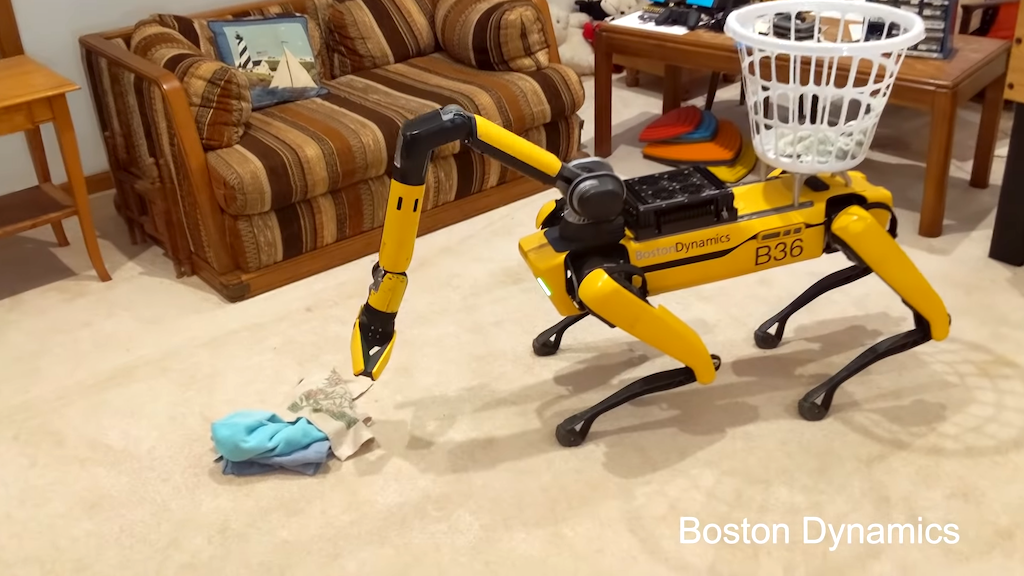
\includegraphics[width=0.8\linewidth]{figs/Spots-Got-an-Arm.png}
    \caption{Boston Dynamics' Spot Mini robot picking up clothes in a living room. These types of complex interactions require the robot to have a semantic understanding of the objects in its environment.}%
    \label{fig:spot-mini}
\end{figure}

In recent years, geometry-based SLAM has achieved high levels of performance in \textit{experimental setups} for localization tasks. Many variants of SLAM algorithms, from ORB-SLAM~\cite{mur-artalORBSLAM2OpenSourceSLAM2017} to Direct Sparse Odometry (DSO)~\cite{engelDirectSparseOdometry2018}, can now run in real-time with high trajectory accuracy. However, they are in general limited by the \emph{static-world} assumption and low-level scene representation as sparse 3D feature points, and thus cannot distill high-level information also known as semantic understanding in scenes and adjust to structured environmental changes.

On the other hand, with progress in deep learning, near real-time semantic perception is achievable powered by efficient Deep Neural Networks (DNNs). There has been explosive progress in object detection and instance segmentation over the past 5 years \cite{renFasterRCNNRealTime2016, heMaskRCNN2018, redmonYouOnlyLook2016} which is underutilized in SLAM. Researchers have started to switch to semantic SLAM taking advantage of off-the-shelf solutions; pioneering research includes SLAM++~\cite{salas-morenoSLAMSimultaneousLocalisation2013}, Fusion++~\cite{mccormacFusionVolumetricObjectLevel2018}, and MaskFusion~\cite{runzMaskFusionRealTimeRecognition2018}. These initial attempts take into consideration semantic segmentation, but typically simply attach DNN frontends to existing SLAM frameworks in an ad hoc fashion. Implementation-wise, they require high-end machines to achieve near real-time performance, or are not available to the community.

\section{Contributions}

\begin{figure}[htbp]
    \centering
    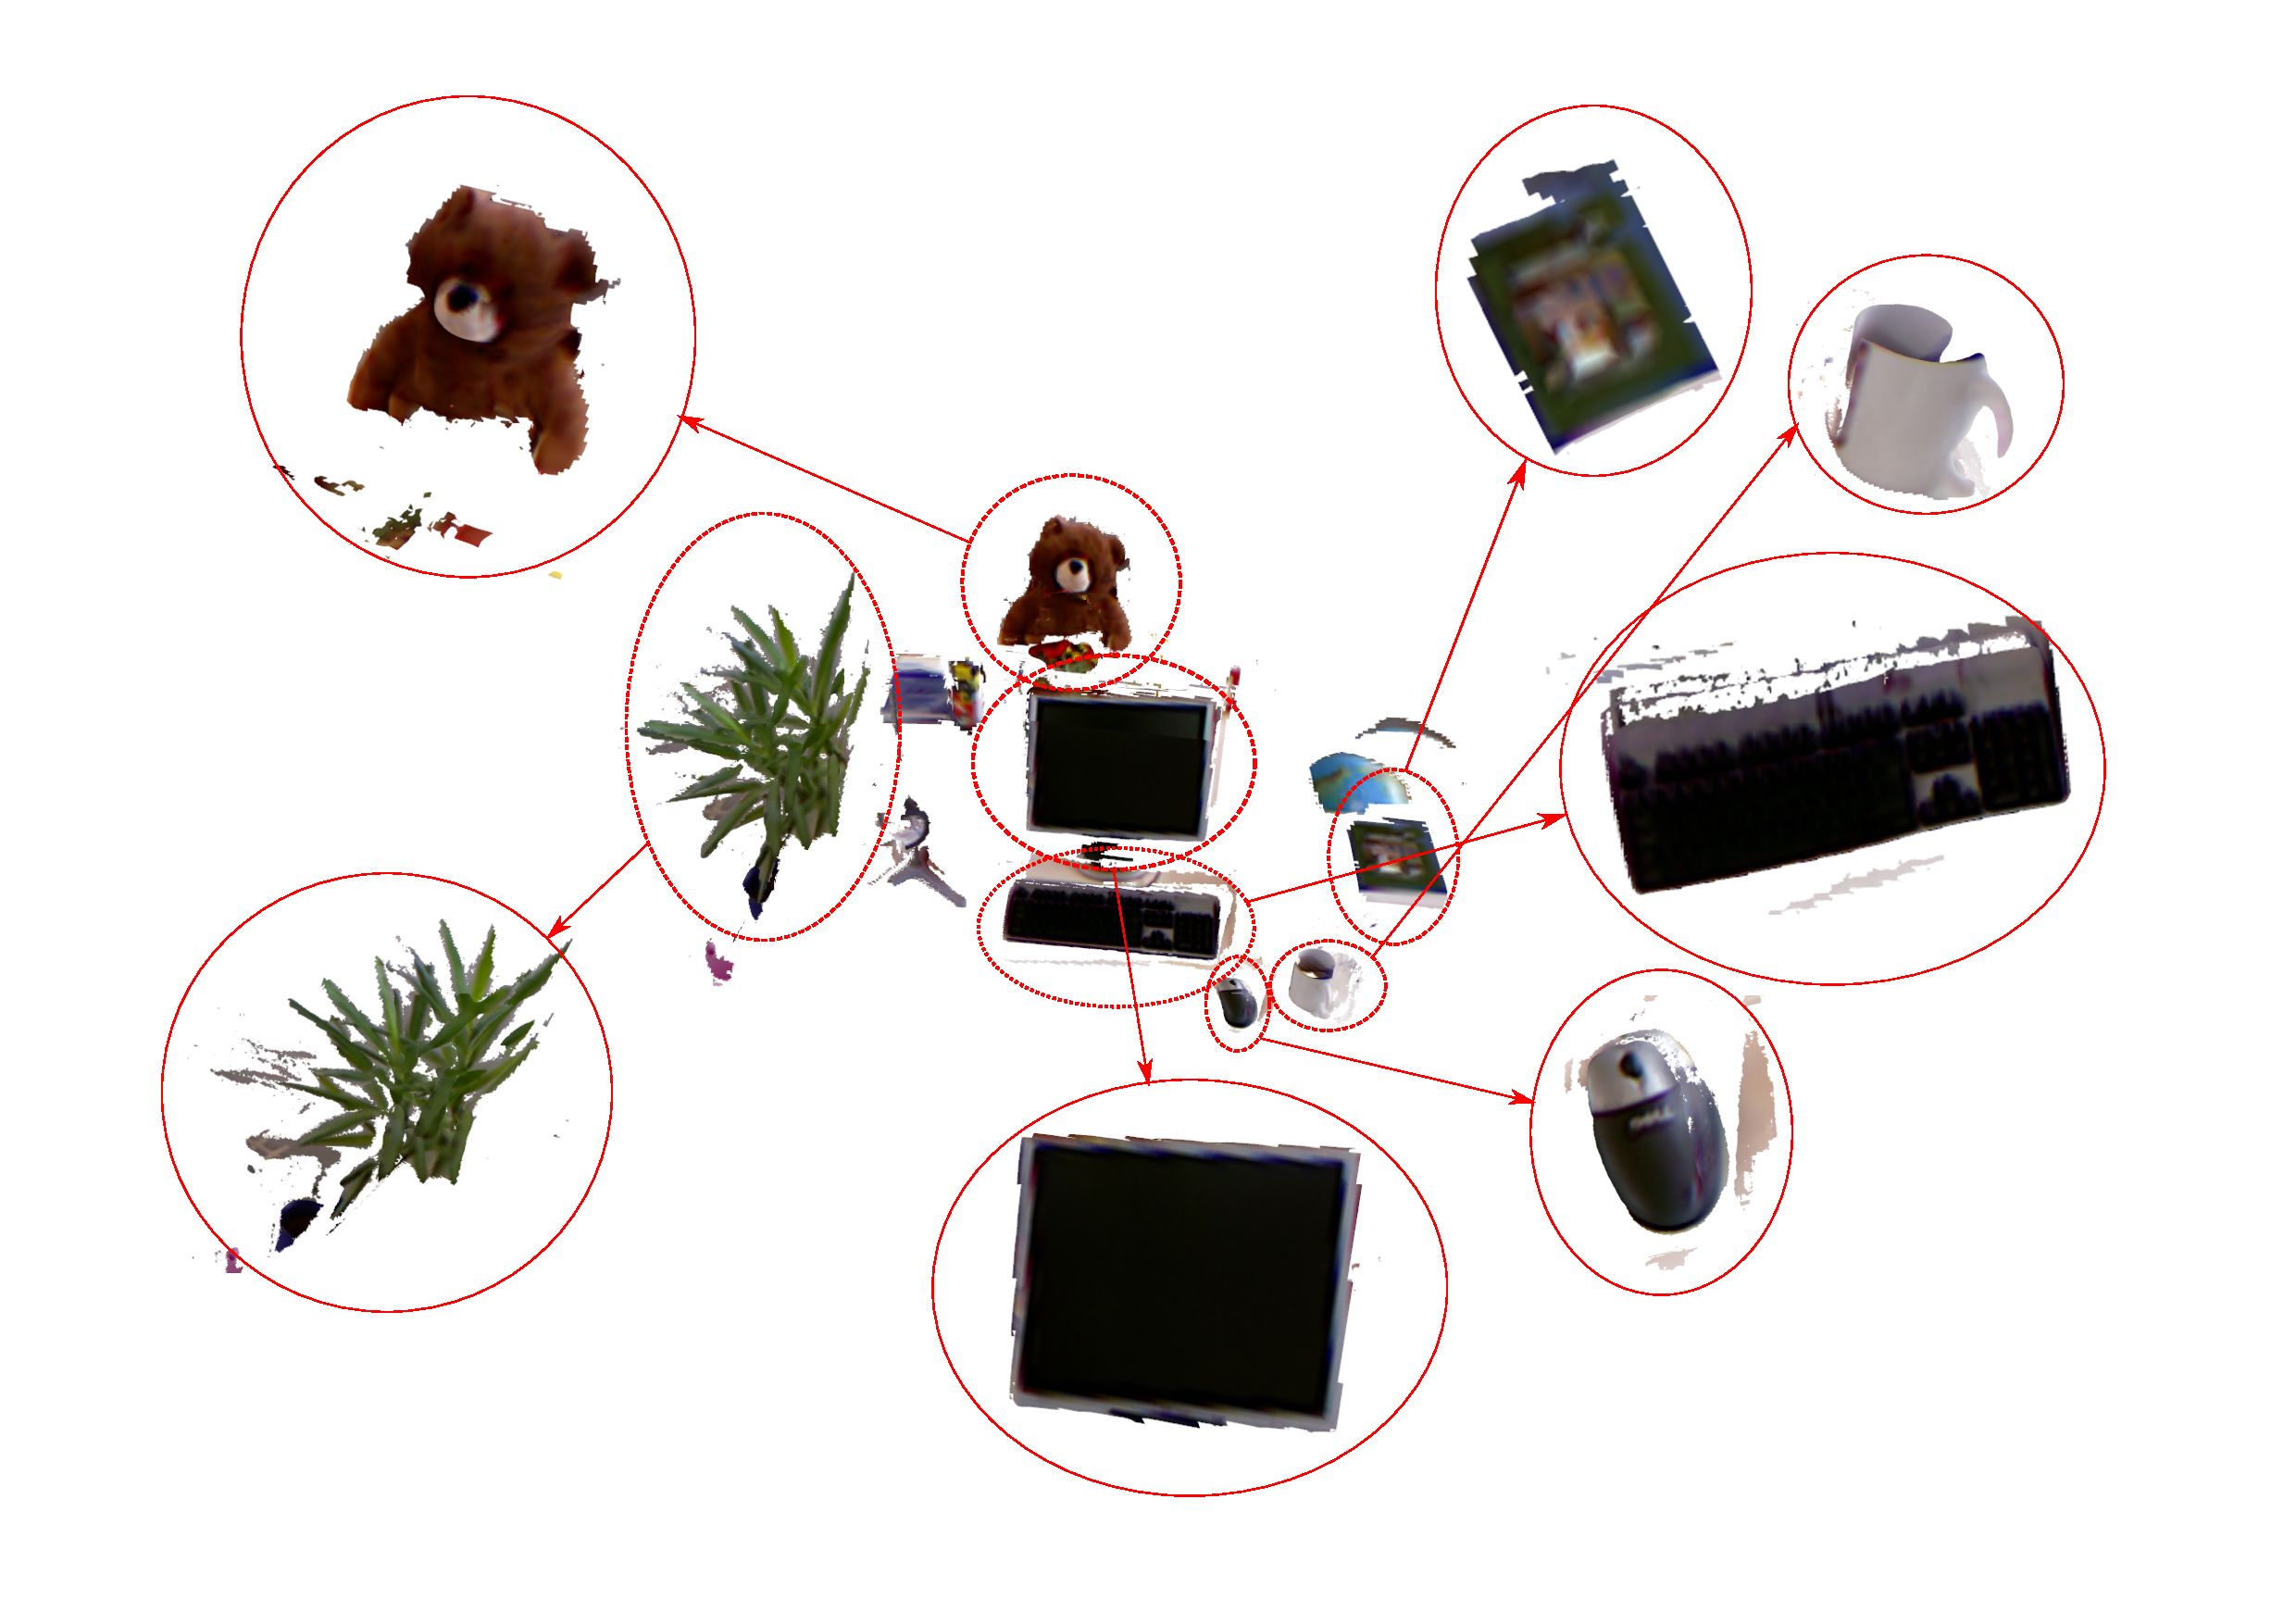
\includegraphics[width=\linewidth]{figs/teaser.pdf}\vspace{-1cm}
    \caption{Reconstruction of \textit{fr2\_xyz} sequence from \emph{tum rgbd} dataset. Our pipeline can reconstruct both camera trajectory and object models in the scene.}
    \label{fig:objectsandscene}
\end{figure}

In this thesis, I present a Compositional and Scalable Object SLAM system that represents an environment as a pose graph of persistent objects. I describe a system, that incrementally improves each associated persistent object landmark through a RGBD Fusion approach, and optimizes the landmarks and the robot trajectory simultaneously to accurately represent an environment. (see Figure~\ref{fig:objectsandscene}).

In implementation, this work fully exploits the power of the modern GPU-based reconstruction pipeline~\cite{dongGPUAcceleratedRobust2019} and object detection frameworks~\cite{kirillovPointRendImageSegmentation2020}, to design an efficient architecture for data exchange without sacrificing the ease of system configuration and build.


This document presents the following core contributions:

\begin{enumerate}
    \item A compositional volumetric rendering method that feeds the most up-to-date model render for RGBD camera tracking;
    \item A hybrid object association method that combines geometric and semantic cues to enable drift-free tracking without an explicit relocalization module;
    \item A scalable, modular, and easy-to-use open source system that runs nearly realtime.
\end{enumerate}

\section{Organization}

In Chapter~\ref{chap:background} we first review some requisite preliminaries and concepts in SLAM, and dense 3D reconstruction.

\noindent In Chapter~\ref{chap:object-slam} we introduce the core SLAM system that forms the major contribution of this thesis. This chapter presents some of the improvements made in the SLAM system with object landmarks, and delineates each component in the pipeline.

\noindent In Chapter~\ref{chap:experiments}, we present some qualitative and quantitative experiments and discussion by comparing against existing state-of-the-art geometric SLAM systems and a few dense semantic SLAM systems.

\noindent Finally, in Chapter~\ref{chap:conclusion}, we conclude the thesis, with some limitations and future directions of research work to improve SLAM systems.


% -*- mode:LaTex; mode:visual-line; mode:flyspell; fill-column:75-*-
\chapter{Background} \label{chap:background}

As eluded to in Chapter~\ref{chap:introduction}, SLAM systems that run on real robots can be crudely divided into \emph{front-end} and \emph{back-end}. This chapter is a primer on algorithms and methods used in the \emph{front-end} and \emph{back-end}.

\section{The Front End}

The robotic paradigm describes the relationship of an agent interacting with its environment through the \emph{sense-plan-act} control loop. SLAM being in the sense paradigm, deals with processing the raw environment sensor readings to a structured representation that can be used in downstream tasks.

The front end deals with data preparation, modeling and data association such that it is amenable to the underlying optimization. More often than not, the choice of front-end is sensor dependent. For instance, many visual SLAM systems that utilize a monocular or stereo camera resort to \emph{feature based}~\cite{qinVINSMonoRobustVersatile2018, loiannoVisualInertialOdometry2016} sparse representations, while RGBD sensor based systems resort to \emph{direct methods}~\cite{newcombeKinectFusionRealtimeDense2011, whelanElasticFusionDenseSLAM2015} that utilize all the pixels in the input frame.

This distinction in the choice of front-end often influences the choice of map representation in a SLAM system. A popular choice with visual SLAM system is to use an \emph{explicit} map representation as a set of 3D points~\cite{mur-artalORBSLAM2OpenSourceSLAM2017} that is \emph{triangulated} from multiple 2D image feature correspondences. On the other hand dense front-end systems rely on \emph{surfel} representations or on volumetric representations such as occupancy grids. More recently, after the seminal work \cite{newcombeKinectFusionRealtimeDense2011}, \emph{implicit} map representations have gained popularity as a candidate representation for RGBD SLAM systems.

In this work, since the focus is on semantic high level object landmarks each represented with implicit representations such as Truncated Signed Distance Function (TSDF) grids, the next section provides a short introduction of this representation.

\subsection{Implicit map representation through TSDFs}

\begin{figure}[htpb]
    \centering
    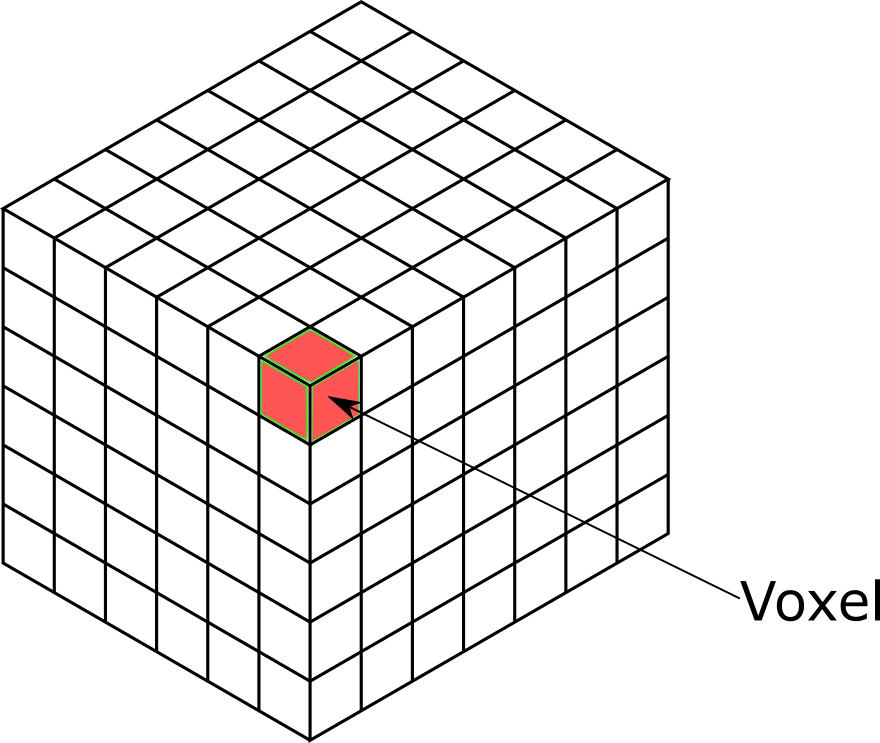
\includegraphics[width=0.5\linewidth]{figs/metric-space-grid.png}
    \caption{An example of metric space in 3D discretized on a computer as a voxel grid.}%
    \label{fig:voxel-grid}
\end{figure}

\emph{Implicit} map representations are fundamentally different from \emph{explicit} map representations. As opposed to point clouds or landmark collections, an implicit map refers to one where the environment is defined through a metric space $\Xv$ (see Figure~\ref{fig:voxel-grid}) and structures in this space are described through an \emph{implicit} function $f : \Xv \rightarrow \Rb$. One example of an implicit function is the log-odds occupancy, resulting directly in occupancy grids \cite{thrunProbabilisticRoboticsIntelligent2005} and \emph{octree} \cite{hornungOctoMapEfficientProbabilistic2013} representations. Another is the signed distance function (SDF) which is relevant for this thesis. Formally, it is defined as follows:

In a metric space $\Xv$ defined with distance $d$, if the surface defined by $\partial \Omega$ demarcates this space into subsets  $\Omegav$ and  $\Omegav^c$, the signed distance function $f$ is defined by
\begin{align}
   f = \begin{cases}
       \phantom{-}d(\xv, \partial \Omegav), &\text{ if } \xv \in \Omegav\\
       -d(\xv, \partial \Omegav), &\text{ if } \xv \in \Omegav^c
   \end{cases}
\end{align}
In particular, for the 3D environment, we have that $\Xv = \Rb^3$ with $d = \|\cdot, \cdot \|_2$, and $\partial \Omega$ corresponds to the zero level set of the signed distance function and represents the surface of objects as a topological space. In simple words, the signed distance function returns the shortest distance of a query point in Euclidean space to its closest point on the surface boundary (see Figure~\ref{fig:2d-sdf}).

\begin{figure}[htpb]
    \centering
    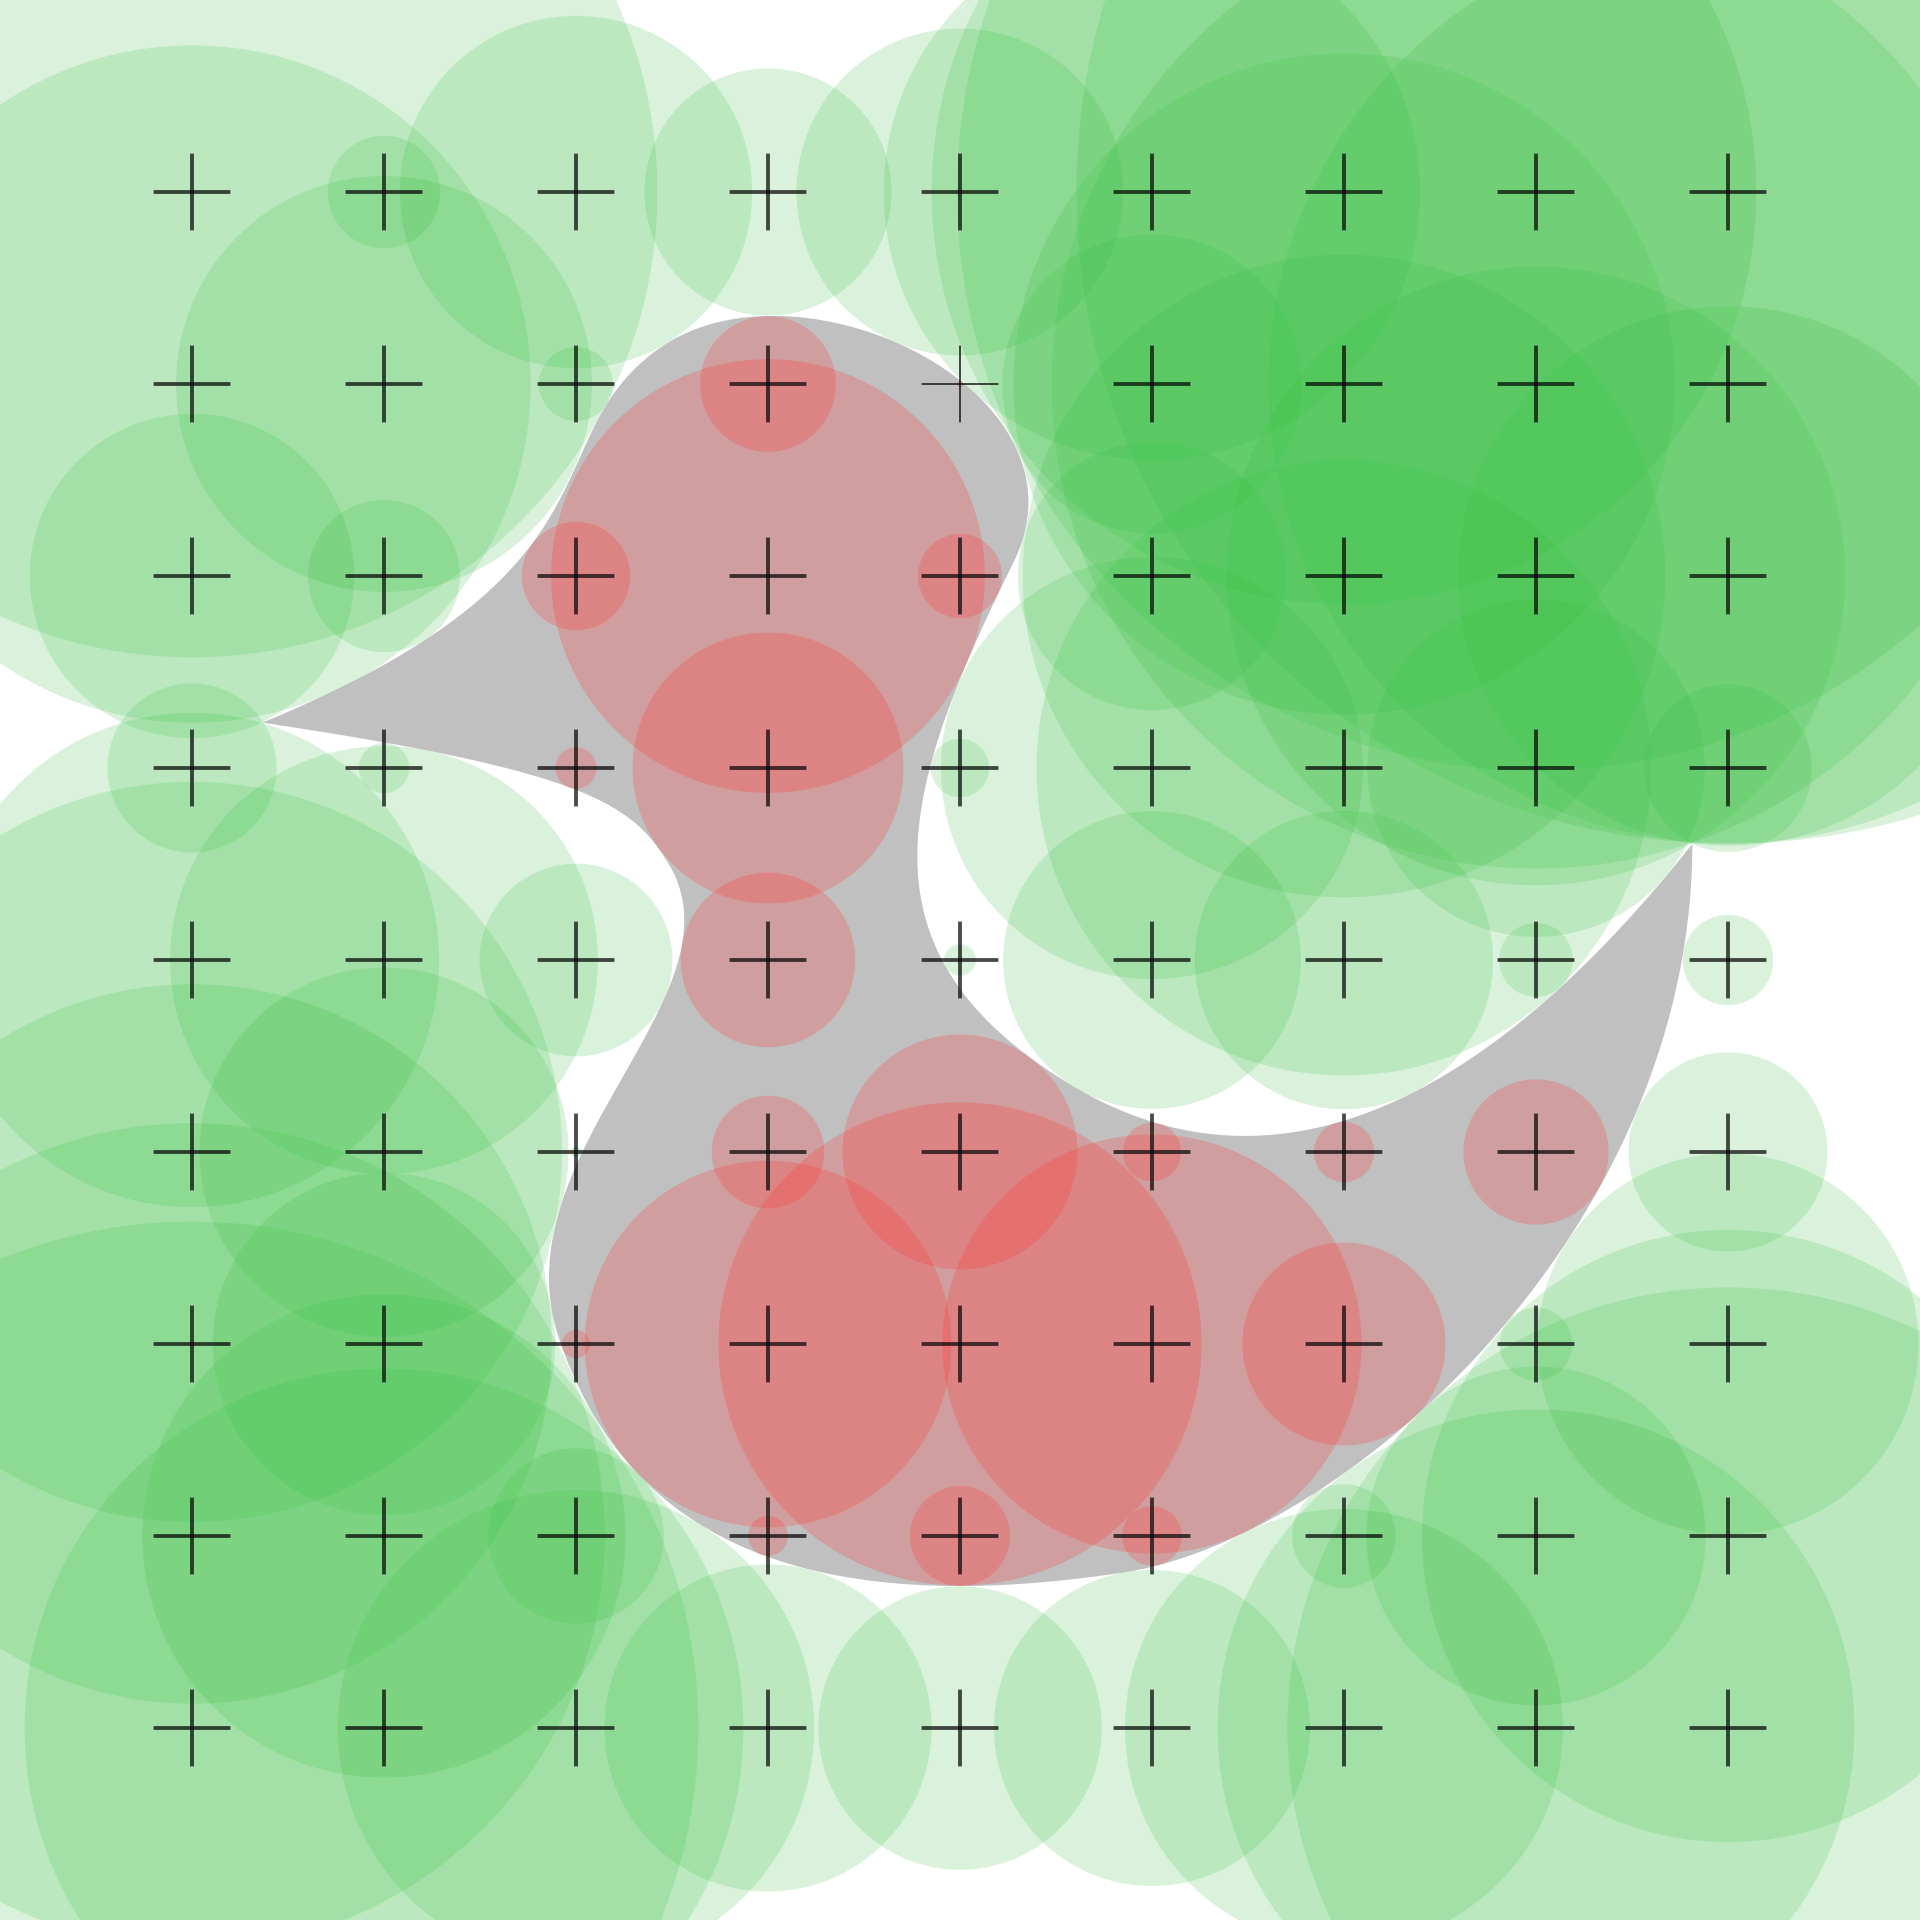
\includegraphics[width=0.5\linewidth]{figs/2d-sdf.png}
    \caption{An illustration of Signed Distance Function for a 2D metric space discretized into pixels (query coordinates '+') (Courtesy: Wikipedia).}%
    \label{fig:2d-sdf}
\end{figure}

\subsubsection{TSDF integration}

A TSDF representation requires a metric volume by design, which is implemented as a volumetric grid $V$, arbitrarily initialised in the world frame $\Tv_W = \Iv \in SE(3)$. Consider a single RGBD frame measurement $\langle \Ic, \Dc \rangle$ that consists of a color ($\Ic$) and depth ($\Dc$) image, at a relative camera pose $\Tv_C^W  = \begin{bmatrix}
    \Rv_C^W & \tv_C^W \\ 0 & 1
\end{bmatrix}\in SE(3)$ with camera intrinsics $\Kv$. To integrate the measurement into the TSDF volume, we project  all the query points $q \in \Rb^3$ of the volume $V$ into the current image as follows:
\begin{align}
    \dot{q}^\prime = (\Tv_C^W)^{-1} \dot{q} \\
    \dot{p} = \lfloor \Kv q^\prime\rfloor
\end{align}
where $\dot{q} = \begin{bmatrix}
    q^\top & 1
\end{bmatrix}^\top$  and similarly $\dot{p}$ denote the homogeneous coordinates in $\Rb^2$ and $\Rb^3$ respectively. $p \in \Zb^2$ is the associated 2D pixel coordinate in the image and $\lfloor \cdot \rfloor$ is the floor function and finds the greatest integer pixel coordinate less than the pixel value in the image. For every matched pixel coordinate, we backproject the associated measurement i.e., the depth value of the pixel $\Dc(p) \in \Rb$ into the volume to obtain a \emph{noisy} 3D surface in the metric space (see Figure~\ref{fig:tsdf-single-image}). This noisy surface is used as the proxy surface against which all query coordinates ($q \in \Zb^3$) in the volumetric grid are evaluated against to obtain their corresponding SDF values as follows:

\begin{align}
    \text{SDF}(q) =  \norm{ \Dc(p) - \frac{1}{\lambda} \|\tv_C^W - q\|_2 }_2
\end{align}

 where $\| \tv_C^W - q \|_2$ is the distance between the query point and the camera center along the camera optical axis, and $\lambda = K^{-1} p$ defines the ray direction for the pixel $p$. This effectively calculates the shortest distance of the query coordinate to the surface.

\begin{figure}[htpb]
    \centering
    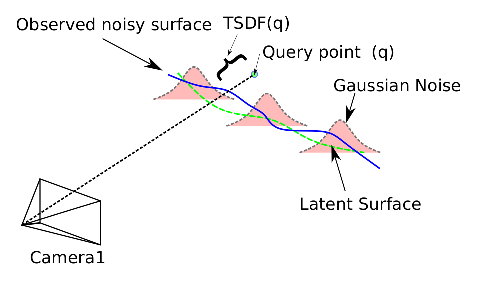
\includegraphics[width=0.6\linewidth]{figs/tsdf-integration-single}
    \caption{Back-projection of associated pixels into the 3D volumetric grid to obtain a noisy surface.}%
    \label{fig:tsdf-single-image}
\end{figure}

This SDF value is truncated such that only a band of SDF values ($+\mu$ to $-\mu$) around the measured surface are computed, to avoid computation of all the query coordinates in the volume.
Similarly, colors from the image can be associated to the query coordinates by unprojection uniquely since a depth image is available.

\begin{figure}[htpb]
    \centering
    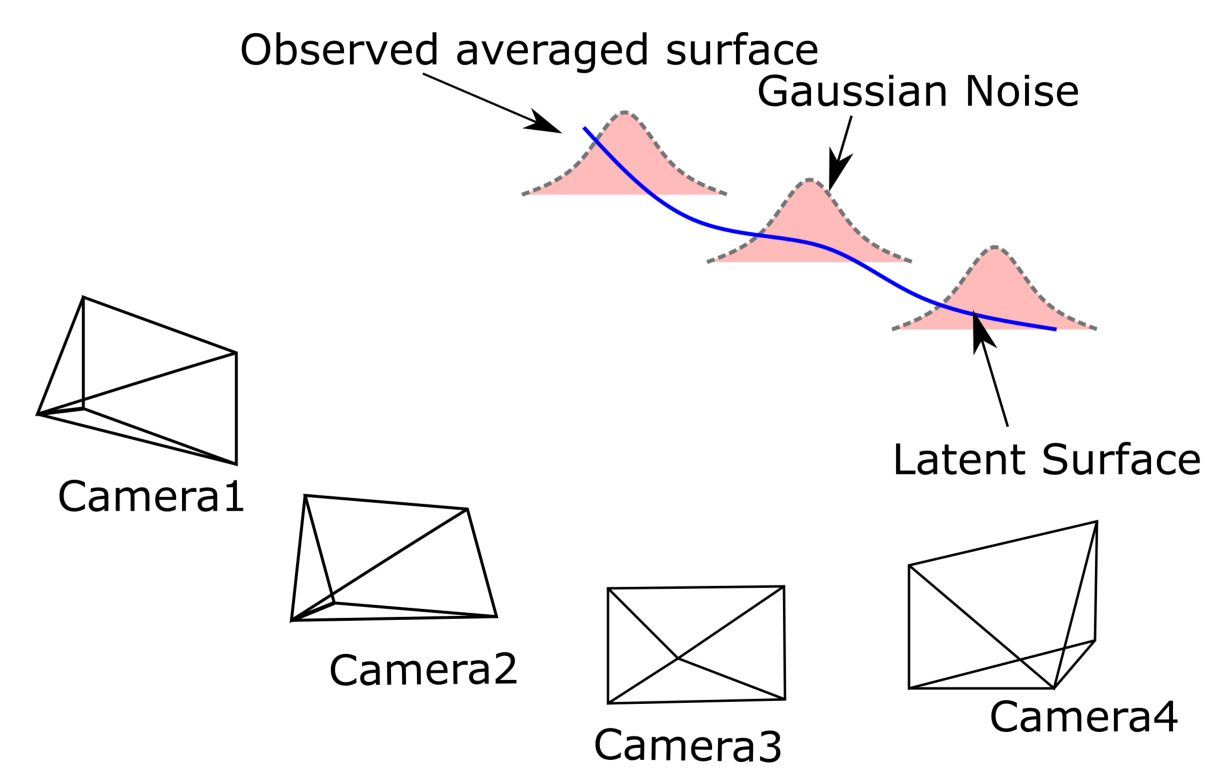
\includegraphics[width=0.5\linewidth]{figs/tsdf-multiple-images.png}
    \caption{On weighted averaging of TSDF values obtained from multiple RGBD measurements, in the limit we converge to TSDF values of the underlying surface.}%
    \label{fig:tsdf-multiple-images}
\end{figure}

Now, when we have multiple RGBD frame measurements $\{\langle \Ic^{(i)}, \Dc^{(i)} \rangle\}_{i=1}^{N}$ with their respective poses $\{ T_{C^{(i)}}^W \}_{i=1}^N$, we can compute TSDF measurements from each individual frame. The global fusion of all these TSDF measurements is then done through weighted average of the TSDF measurements for each query coordinate $q \in \Rb^3$ over the camera frame sequence as follows:
\begin{align}
    d &= \phi(\text{SDF}(q)) \\
    \text{TSDF}_k(q) &= \frac{\text{TSDF}_{k-1}(q) + d}{W(q) + 1} \\
    W(q) &= W(q) + 1
\end{align}
where $\phi$ truncates the $\text{SDF}$ computed for the frame being integrated, and $W(q)$ corresponds to the maintained weight for every voxel coordinate in the volume grid. This integration process intuitively results in evaluation of the SDF values for the query coordinates with the expected surface (mean of the TSDFs) from all the incorporated RGBD measurements (see Figure~\ref{fig:tsdf-multiple-images}).


In general, the integration process can also be applied to the color values, where the colors are averages elementwise, with the incoming stream of images.

\subsubsection{TSDF Rendering}

TSDF Rendering is the process of generating a virtual depth and color image given a camera pose $\Tv_C^W$ and TSDF volume grid $V$. The previous subsection assumed access to camera poses for global TSDF fusion, but in an actual SLAM setting camera poses are computed in the loop typically through iterative closest point (ICP)~\cite{rusinkiewiczEfficientVariantsICP2001} registration. TSDF Rendering is the intermediate step that generates a virtual image that the incoming camera frame is registered against (also called \emph{frame to model} registration~\cite{newcombeKinectFusionRealtimeDense2011}). (details in \S\ref{subsec: tracking})

Rendering is accomplished by marching a ray per pixel of the virtual frame into the global TSDF volume which encodes surfaces as the zero level set (zero crossing). For a given pixel $p \in \Zb^2$, once again the camera ray can be computed as
\begin{align*}
    \rv = \Tv_C^W \Kv^{-1} \dot{p}.
\end{align*}
\noindent We then march along the ray from the minimum depth supported by the camera (usually assumed to be $0.1$m) to a max depth value defined by the supported camera range (around 5m to 8m for Microsoft Kinect), or until we find a zero crossing. Typically this process is sped up by skipping marching along the ray, and using a step size $< \mu$, the truncation threshold. Once a zero crossing has been found, the depth value can be further refined by trilinear interpolation. (details in~\cite{newcombeKinectFusionRealtimeDense2011})

\subsection{TSDF Limitations}

Based on the discussion of TSDF for map representation in SLAM, the following limitations might be apparent to the keen reader.
\begin{enumerate}
    \item \textbf{TSDF representation is memory intensive:} A naive TSDF representation, utilizes a 3D volumetric grid to represent the scene -- typically  a voxel grid of resolution $512^3$ covering a bounded volume of about $4m^3$. This makes the entire system very memory intensive. Later works such as Voxel Hashing~\cite{niessnerRealtime3DReconstruction2013} and OctoMap \cite{hornungOctoMapEfficientProbabilistic2013} have tried to ameliorate this issue. In our implementation, we utilize this spatial hashing based TSDF implementation based on \cite{dongGPUAcceleratedRobust2019} to achieve memory efficiency.
    \item \textbf{TSDFs are computationally intensive:} During integration of an incoming frame, all pixels that are projectively associated to the 3D query coordinates are updated requiring about $640\times 480 = 307200$ operations for a VGA resolution image. Similarly, during TSDF rendering, each pixel to be rendered requires at most $\frac{\|d_{\max} - d_{\min}\|_2}{\mu}$ evaluations, where $\|d_{\max} - d_{\min}\|_2$ is the maximum ray length, and $\mu$ is the TSDF truncation width. Therefore, ray-casting is typically the most computationally intensive step in any dense RGBD SLAM system. Observing that each pixel is updated independent of others, a GPU can (and is) used to parallelize all TSDF operations, to obtain realtime operation.

\begin{figure}[htpb]
    \centering
    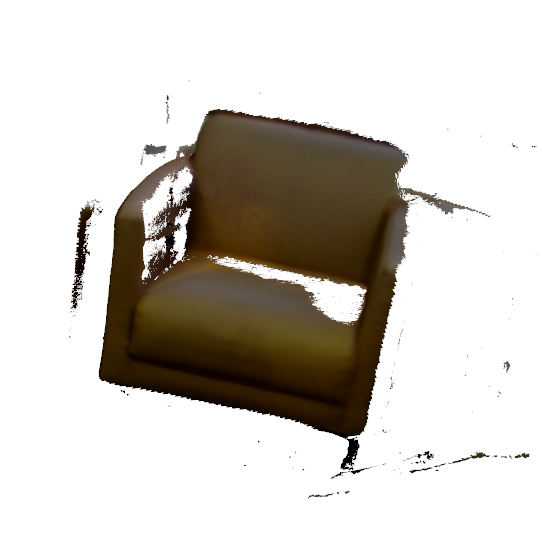
\includegraphics[width=0.4\linewidth]{figs/chair-landmark.png}
    \caption{An example of dense high level landmark in our SLAM system.}%
    \label{fig:chair-landmark}
\end{figure}

    \item \textbf{Cannot easily smooth noisy pose estimates:} It is not easy to correct noisy pose estimates with implicit models, and therefore most early systems employed only a filtering based integration \cite{newcombeKinectFusionRealtimeDense2011}. This is because to correct for a noisy pose estimate in retrospect requires the expensive operation of subtracting the weighted TSDF values in the global volume from the appropriate coordinates and re-integrating the volume with corrected TSDF values \cite{daiBundleFusionRealtimeGlobally2017}. \cite{whelanKintinuousSpatiallyExtended} used submaps to subvert this problem, however with large TSDF volumes as submaps there are still locally noisy measurements that are not corrected for. In our method, since we use a TSDF representation only for landmark objects, we reap the benefits of explicit representation, where the whole landmark pose can be optimized, but each landmark provides a dense and appealing representation. (see Figure~\ref{fig:chair-landmark})
\end{enumerate}

\section{The Back End}

The back end is responsible for generating a reasonable explanation in the state variables given the abstract sensor measurements and data associations from the front end. As opposed to filtering based methods such as Kalman Filter, more recently smoothing formulations based on matrix factorization have provided exact solutions in the linear case, and approximate but good solutions in non-linear case by adding the entire trajectory into the optimization problem while simplifying the solution~\cite{kaessIncrementalSmoothingMapping}. In this section, I review the batch smoothing formulation that is quite common in graph based SLAM back-ends today~\cite{grisettiTutorialGraphBasedSLAM, dellaertFactorGraphsRobot2017}.

\subsection{SLAM and Non-Linear Least Squares}

\begin{figure}[htpb]
    \centering
    \includegraphics[width=\linewidth]{figs/factor-graph-background}
    \caption{(a) A factor graph typical for SLAM and (b) the explicit Bayes net for the factor graph in (a). Note the Markovian conditional independences between measurements, given the state variables.}%
    \label{fig:factor-graph}
\end{figure}

As introduced in Chapter \ref{chap:introduction}, by treating the robot states and landmarks as random variables given measurements, the SLAM problem can be treated as the maximum a posteriori (MAP) estimation of robot and landmark states. Now, consider a collection of robot state variables $\Xc \triangleq \{ \xv_t \}_{t=1}^{T}$, and a collection of landmarks $\Lc \triangleq \{ \ell_m \}_{m=1}^{M}$, and set of measurements $\Zc \triangleq \{\{\zv_n \}_{n=1}^{N}, \{\zv_t\}_{t=1}^{T}\}$ including both landmark and odometry measurements respectively, then the MAP estimation is given as
\begin{align}
    \Xc^*, \Lc^* = \argmax_{\Xc, \Lc} p(\Xc, \Lc | \Zc) = \argmax_{\Xc, \Lc} p(\Zc | \Xc, \Lc) p(\Xc, \Lc) \label{eq:map}
\end{align}
While MAP estimation is known to be NP-Hard in general, by assuming reasonable conditional independences between the associated variables (see Figure~\ref{fig:factor-graph}), i.e., by making the markovian assumption on the state variables, and observing that measurements are local, we can write the joint probability in \ref{eq:map} as follows:
\begin{align}
    p(\Xc, \Lc, \Zc) &= p(\xv_0) \prod_{n=1}^{N} p(\zv_n | \xv_{\alpha_n}, \ell_{\beta_n}) \prod_{t=1}^{T} p(\zv_t | \xv_{t-1}, \xv_{t})\nonumber\\
    \log p(\Xc, \Lc, \Zc) &= \log p(\xv_0) + \sum_{n=1}^{N} \log p(\zv_n | \xv_{\alpha_n}, \ell_{\beta_n}) + \sum_{t=1}^{T} \log p(\zv_t | \xv_{t-1}, \xv_{t})
\end{align}
Note, that the above problem assumes known \emph{data association} between measurements $\zv_n$ of landmark $\ell_{\beta_n}$ at a robot pose $\xv_{\alpha_n}$as $\Dc := \{(\alpha_n, \beta_n)\}_{n=1}^{N}$ \cite{bowmanProbabilisticDataAssociation2017}.
Now as is typical in SLAM, we assume Gaussian measurement noise in each of the measurements i.e.,
\begin{align}
    \zv_0 &= \xv_0 + \nuv_0\\
    \zv_n &= h_n(\xv_{\alpha_n}, \ell_{\beta_n}) + \nuv_n\\
    \zv_t &= h_t(\xv_{t-1}, \xv_t) ~+ \nuv_t
\end{align}
Where $\nuv_n$ and $\nuv_t$ are the intrinsic noise in the respective measurements, each distributed as zero mean noise with respective covariances $\Sigma_n$ and $\Sigma_t$. Also note that we added a phantom measurement $\zv_0$ to constrain the first pose with an empirically chosen small covariance $\Sigma_0$. On writing down the probability distributions for each of the Gaussian noise terms we have the following:
\begin{align}
    p(\xv_0) &\propto \exp\{ \|\zv_0 - \xv_0\|^2_{\Sigma_0}\}\\
    p(\zv_n | \xv_{\alpha_n}, \ell_{\beta_n}) &\propto \exp\{ \|\zv_n - h_n(\xv_{\alpha_n}, \ell_{\beta_n})\|^2_{\Sigma_n}\}\\
    p(\zv_t | \xv_{t-1}, \ell_{t}) &\propto \exp\{ \|\zv_t - h_n(\xv_{t-1}, \ell_{t})\|^2_{\Sigma_t}\}
\end{align}
Observe that
\begin{align}
    \Xc^*, \Lc^* &= \argmax_{\Xc, \Lc} p(\Xc, \Lc, \Zc) = \argmin_{\Xc, \Lc} - \log p(\Xc, \Lc, \Zc)
\end{align}
Now writing the joint probability using the factorized measurement distributions we have
\begin{align*}
    \Xc^*, \Lc^* = \argmin_{\Xc, \Lc} \Bigg \{ \| \zv_0 - \xv_0 \|_{\Sigma_0}^2 + &\sum_{n=1}^{N} \| \zv_n - h_n(\xv_{\alpha_n}, \ell_{\beta_n}) \|_{\Sigma_t}^2 + \\&\sum_{t=1}^{T}\| \zv_t - h_t(\xv_{t-1}, \xv_{t}) \|_{\Sigma_n}^2 \Bigg \}
\end{align*}
If we generalize the different types of measurements in the system as $h_i(\Xv_i)$, and subsume the landmarks and state variables into a single state vector $\Xc$ then we may write the above as:
\begin{align}
    \Xc^* = \argmin_{\Xc} \Bigg \{ &\sum_{i=1}^{N} \| \zv_i - h_i(\Xv_i) \|_{\Sigma_i}^2 \Bigg \} \label{eq:least-squares}
\end{align}
The above minimization is a non-linear least squares optimization which is typically solved by iteratively linearizing the measurement models and solving a series of linear approximations to the problem to approach a local minima solution for landmark and robot latent state variables.

\subsection{Iterative Linearization and Gauss Newton}


Consider a single non-linear measurement $h_i( \cdot )$, then by Taylor's expansion, we can linearize the measurement at a linearization point $\Xv_i^{(0)}$ as follows (see Figure~\ref{fig:taylor}):
\begin{align}
    h_i(\Xv_i) \approx h_i(\Xv_i^{(0)}) + \frac{\partial h_i}{\partial \Xv_i} \Bigg |_{\Xv_i^{(0)}} (\Xv_i - \Xv_i^{(0)})
\end{align}
If we define the jacobian as $\Jv_i \triangleq \frac{\partial h_i}{\partial \Xv_i} \Big|_{\Xv_i^{(0)}}$, and $\Delta_i \triangleq (\Xv_i - \Xv_i^{(0)})$ and substitute in the general non-linear least squares objective \ref{eq:least-squares}:

\begin{figure}[htpb]
    \centering
    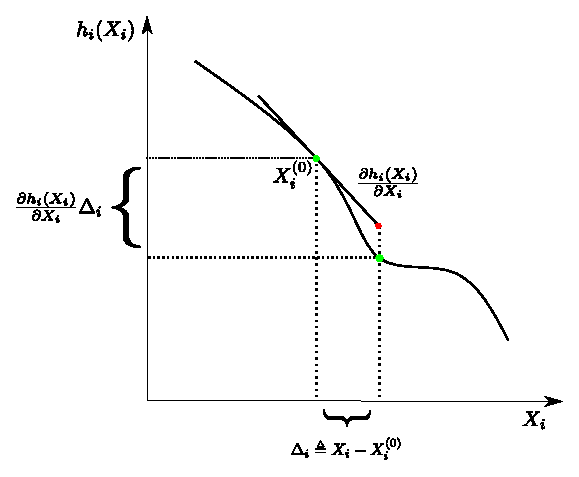
\includegraphics[width=0.5\linewidth]{figs/linearization}
    \caption{Illustration of linearization using Taylor's expansion.}
    \label{fig:taylor}
    \vspace{-1em}
\end{figure}
\begin{align}
    \Delta^* = \argmin_{\Delta}\sum_{i} \| \{\zv_i - h_i(X_i^{(0)})\} - \Jv_i \Delta_i \|_{\Sigma_i}^2
\end{align}
where $\qv_i \triangleq \zv_i - h_i(\Xv_i^{(0)})$ is the prediction error at the linearization point, and $\Delta^*$ is the solution to the locally linearized problem. Now we may write the least squares objective as:
\begin{align}
    \Delta^* &= \argmin_{\Delta}\sum_{i} \| \qv_i - \Jv_i \Delta_i \|_{\Sigma_i}^2 = \argmin_{\Delta}\sum_{i} (\qv_i - \Jv_i \Delta_i)^\top \Sigma_i^{-1} (\qv_i - \Jv_i \Delta_i)\\
             &=  \argmin_{\Delta}\sum_{i} \left\{\Sigma_i^{-1/2}(\qv_i - \Jv_i \Delta_i)\right\}^\top \left\{ \Sigma_i^{-1/2} (\qv_i - \Jv_i \Delta_i)\right\}\\
             &= \argmin_{\Delta}\sum_{i} \| \bv_i - \Av_i \Delta_i \|_2^2 = \argmin_{\Delta} \| \bv - \Av \Delta\|_2^2
\end{align}
By writing $\bv_i = \Sigma_i^{-1/2} \qv_i$ and $\Av_i = \Sigma_i^{-1/2} \Jv_i$ and then collecting them in the vector $\bv$ and matrix $\Av$ respectively, we obtain the standard least squares problem, that can then be solved using \emph{normal equations}.

The above solution gives us the local update $\Delta^*$ for a linearization point $\Xv^{(0)}$. To solve a non-linear problem, we solve for local updates iteratively as in Algorithm~\ref{gauss-newton}.


\begin{algorithm}[htpb]
\begin{algorithmic}[1]
    \Procedure{Gauss Newton}{$g(\Xv), \Xv^{(0)}$}
    \State $d = \text{threshold}$
    \For{t = 0 to N}
        \State $\Av, \bv \leftarrow$ Linearize$(g(\Xv))$ at $\Xv^{(t)}$
        \State $\Delta^* \leftarrow (\Av^\top \Av)^{-1} \Av^\top \bv$ \Comment{using QR or Cholesky factorization}
        \State $\text{temp} \leftarrow \Xv^{(t)} + \Delta^*$
        \If{$g(\text{temp}) < g(\Xv^{(t)})$}
            \State $\Xv^{(t+1)} \leftarrow \text{temp}$
            \If{$g(\Xv^{(t+1)}) - g(\Xv^{(t)}) < d$}
                \State \textbf{break}
            \EndIf
        \EndIf
    \EndFor
    \State \Return $\Xv^{(t)}$
\EndProcedure
\end{algorithmic}
\caption[short caption]{Iterative Non-linear optimization}
\label{gauss-newton}
\end{algorithm}


A more detailed treatment of sophisticated non-linear optimization algorithms in the context of SLAM is provided in \cite{dellaertFactorGraphsRobot2017}.

\subsection{Discussion and Limitations}

We noted earlier that MAP inference on the factor graph for the SLAM setting is tractable due to the inherent local structure of the factor graph. This structure appears in the sparsity of the measurement Jacobian $\Av = \Sigma^{-1/2} \Jv$ with number of rows equal to the number of measurements in the graph (number of factors) and the number of columns equal to the number of state variables to be solved. The non-linear least squares optimization is solved efficiently using matrix factorization methods such as QR factorization and Cholesky factorization (equivalent to variable elimination on the factor graph~\cite{dellaertSquareRootSAM2006}). Further improvement in performance can be gained by reordering the measurements using methods such as COLAMD \cite{davisAlgorithm8xxCOLAMD} which consequently reduces fill in in the matrix during computation.

Nevertheless, for an online system with this formulation matrix factorization needs to be performed with a new graph when new measurements are added, resulting in wasted computation to resolve all the entries in the matrix. Later work has made progress on incremental solvers for SLAM, that are able to update the solution iteratively for non-linear systems and provide linearization point management, as well as careful updation of older variables based on the current estimate. As this thesis does not directly use incremental solvers, the reader is directed to \citet{kaessISAM2IncrementalSmoothing2012}

For implicit mapping representations, however, it is unclear how they are to be represented as landmark variables, and how updates to the landmark state variables are to be propagated in the map. In this thesis, we show that representing the map as a collection of high level objects, each represented with implicit representation and corresponding to a landmark variable in the optimization is a good strategy, and benefits the SLAM in multiple facets. Each object is represented with a spatially hashed TSDF volumetric grid \cite{prisacariuInfiniTAMV3Framework2017} \cite{niessnerRealtime3DReconstruction2013} \cite{dongGPUAcceleratedRobust2019} that is not updated in the back end optimization process. Instead, since the object is rigid, optimizing the pose of the base frame attached to it suffices.
\clearpage
% In theory implicit map representations provide a method for water tight  reconstructions that are visually appealing, and in general more detailed when compared to feature based methods (see Figure Figure~\ref{fig:}), however these methods typically do not employ smoothing based back ends, and therefore are unable to correct for noisy pose estimates in retrospect. This is because, it is not easy to make a correction to an integrated measurement in the TSDF representation. In particular, to correct a single pose estimate, the measurement that had been integrated into the global TSDF has to be removed by subtractingthe corresponding TSDF value from the affected 3D query coordinates, and then re-integrating the new measurement appropriately.



\chapter{SLAM with Object Landmarks} \label{chap:object-slam}

In this chapter I present a SLAM formulation with object landmarks, which is scalable to medium sized indoor scenes and is robust to data association errors through the use of semantic information. Further I also present a compositional rendering method to render an accurate model frame at any given time during operation to propagate updated information to the front end in turn providing better initialization for the back end. This work is similar in spirit to a line of work started by \cite{salas-morenoSLAMSimultaneousLocalisation2013}. In this thesis however, the focus is on accurate trajectory estimation as well as object reconstruction. In essence, our work can be regarded as a bridge between feature based SLAM methods and dense SLAM methods.

\section{Related Literature}

In this section we review relevant literature in two aspects: classical geometry-based SLAM, and the application of deep semantic object detection in SLAM.
% Typically, SLAM methods incorporate semantics in two ways: (1) \textit{Loosely coupled}, where semantics are used post a completely independent map generation step. For instance, \cite{mccormac2017semanticfusion} generates a semantic map by fusing 2D segmentations in a post-processing step through bayesian updates, and \cite{grinvald2019volumetric} proposes a mapping scheme given camera trajectory to fuse geometric segmentation with Convolutional Neural Network (CNN) segmentations (2) \textit{Tightly coupled} where semantics are used directly to jointly optimize the map and camera trajectory. This tightly coupled treatment is called \textit{Object level SLAM}.

\subsection{Geometry-based SLAM}
\subsubsection{Problem formulation and pose optimization}
Modern geometry-based SLAM systems can be generally classified into \textit{feature-based} and \textit{direct} methods.
%
Feature-based SLAM systems ~\cite{mur-artalORBSLAM2OpenSourceSLAM2017, kleinParallelTrackingMapping2007} usually maintain a collection of sparse 3D \textit{point landmarks} corresponding to hand-crafted feature \textit{keypoints} detected in 2D images. In order to correct accumulated \textit{pose} error, \textit{i.e.,} drift, these methods resort to bundle adjustment \cite{triggsBundleAdjustmentModern2000} that jointly minimizes reprojection error between \textit{landmarks} and 2D \textit{keypoints} via \textit{pose} optimization. While being accurate in estimating trajectory, these approaches only come with sparse 3D maps that are less interpretable for visualization and recognition.
%
Direct SLAM~\cite{engelLSDSLAMLargeScaleDirect, engelDirectSparseOdometry2018} on the other hand, relies on pixel-wise projective data association between frames for odometry. Given relative poses between certain keyframes, pose graphs~\cite{dellaertFactorGraphsRobot2017} are formulated and optimized to obtain globally consistent poses without landmark constraints.

Our approach can be regarded as a bridge between the two approaches. We replace point landmarks with objects in feature-based SLAM. As a result, since pose constraints attached to objects can naturally replace reprojection error, we may directly convert such a landmark-pose constraint optimization to pose graph optimization (PGO).

\subsubsection{Map representation}
For \textit{dense} scene reconstruction, the volumetric Truncated Signed Distance Function (TSDF)~\cite{curlessVolumetricMethodBuilding1996} representation has been adopted and improved in several \textit{direct SLAM} frameworks. KinectFusion~\cite{newcombeKinectFusionRealtimeDense2011} introduced a plain $512^3$ grid for small scenes and objects. VoxelHashing~\cite{niessnerRealtime3DReconstruction2013} designed spatial hashing to scale this data structure to larger scenes. Similar implementations are available in CPU/GPU in the modern Open3D framework~\cite{zhouOpen3DModernLibrary2018, dongGPUAcceleratedRobust2019}, and we adopt this representation due to its ease of use.

\subsection{Object instance segmentation and object-based SLAM}
\subsubsection{Object instance segmentation}
In recent years, \textit{Region proposal} based Convolutional Neural Networks (R-CNN) \cite{renFasterRCNNRealTime2016} have established themselves as de-facto standards for object \textit{instance segmentation} from images. Amongst the literature, \textit{Mask-RCNN}~\cite{heMaskRCNN2018} and \textit{PointRend}~\cite{kirillovPointRendImageSegmentation2020} are the best off-the-shelf solutions.
In this work, we use \textit{PointRend} \cite{kirillovPointRendImageSegmentation2020}, which shows significant improvement over \cite{heMaskRCNN2018} by reformulating the mask generation as a rendering problem. In essence, this formulation is consistent with our tracking via compositional rendering module.

\subsubsection{Object-based SLAM}
Applying aforementioned DNNs on 2D images, several works for RGB-D and monocular SLAM have attempted to incorporate object instance detection. CubeSLAM~\cite{yangMonocularObjectPlane2019} and QuadricSLAM~\cite{nicholsonQuadricSLAMDualQuadrics2019} fit cuboids and quadrics, respectively, to detected objects to generate parameterized object landmarks. While improving the localization accuracy compared to baselines, these methods fail to densely map objects. \textit{MaskFusion}~\cite{runzMaskFusionRealTimeRecognition2018} adds labels to oriented point clouds and supports dense object visualization, but does not maintain persistent objects globally in a graph. \textit{Fusion++}~\cite{mccormacFusionVolumetricObjectLevel2018}, on the other hand, supports persistent dense reconstruction from fixed size $64^3$ voxel grids, yet is sensitive to voxel size tuning and may fail to adapt to objects at varying scales.
Our system utilizes scalable voxel grids that do not require much tuning to adjust to object scales. With a seamless CPU to GPU memory transfer implementation, larger environments can also be handled on-the-go.

% In this paper, we demonstrate an object graph formulation for simultaneous dense object reconstruction and accurate camera tracking, leveraging significant improvements in Deep Learning towards Object Detection and Object instance segmentation.


%and \citet{runz_maskfusion_2018} that propose object based representations for a scene. However, \cite{fusionPP} is based on unscalable discrete voxel grids, and uses lower resolution objects of $64^3$ to run feasibly, while \cite{runz_maskfusion_2018} is a surfel based method to track multiple objects and forgoes a factor-graph formulation and .
%More recently, \citet{xu2019mid}, proposes an octree datastructure, and utilizes a joint weighted photometric and geometric dense tracking similar to ours. This paper, however, focuses on tracking dynamic objects, and does not utilize a \textit{factor-graph} to jointly optimize camera, and \textit{correct} object poses.
% R-CNNs extract multiple region proposals, and individually classify and score the predictions to obtain labels and detection scores respectively. More recently, \citet{he2017mask} adds a parallel \textit{mask head} to generate object mask using Fully convolutional networks (FCN). Another line of work \cite{redmon2016you} predicts object bounding boxes directly by dividing an image into blocks and predicting probabilities.

% For directly segmenting \textit{3D data}, sparse convolution~\cite{4Dspatiotempro} and Key point convolution~\cite{kpconv} has started to gain attention in the community for its success on non-uniform point cloud data.

%In our work, we choose object detectors for images rather than point cloud, since we take RGB-D data as raw input, and data association for objects from 2D is easier to obtain and update given depth maps and poses.

%\subsection{Object-based SLAM}
%\textbf{Sparse Feature based methods}. These approaches use object detection as opposed to object instance mask segmentation, to instantiate oriented 3D objects and fit cuboids \cite{yang2019cubeslam} or Quadrics \cite{quadric_slam}. They handle data association either by grouping detected keypoints into semantic labels, or assume known associations and define an Intersection-over-Union (IoU) overlap based error for optimization respectively. Although, these methods show improvement over baselines, they do not focus on object reconstruction fidelity. In contrast, our work uses a dense Hash-table based scalable volume data structure, which allows for accurate object reconstructions.

% \textbf{Direct dense methods}. SLAM++ %\cite{salas-moreno_slam_2013} was an early attempt towards SLAM with 3D object landmarks, that used a dense object representation. This method employed a dictionary of object descriptors generated through only geometric cues of each object model for data-association, and attempted camera trajectory optimization through multiple Frame to model ICP refinement between the live frame and \textit{each} detected object model. Further, a major limitation was that, it required pre-processed high quality mesh models of the expected objects in the scene prior to operation.

% The problem of high-fidelity 3D reconstruction has received substantial attention over the years. Key to high-quality 3D reconstruction is the choice of underlying representation for fusing sensor measurements of different modalities. Thus, most of the research on achieving globally consistent 3D models at scale uses the RGB-D input that encapsulates the semantic as well as geometric (depth) information simultaneously. ~\citet{choi2015robust} proposes a framework that uses RGB-D input to generate a very high-fidelity reconstruction of indoor scenes. They provide globally consistent models by optimizing across the entire pose trajectory. However, their approach requires offline processing and access to all the input frames resulting in hours of processing time, meaning real-time viability of refinement of reconstructed areas is almost impossible. Such joint global registration of multiple partially overlapping surfaces has also been considered by other works~\cite{huber2003fully,theiler2015globally}. To bridge this gap, this work proposes an object-centric pipeline for data association that reduce the expensive computational cost in registration.
% ~\citet{kinectfusion}'s seminal work KinectFusion introduced a new method and made RGBD reconstructions feasible. The key insight was to incorporate frame-to-model tracking as opposed to frame-to-frame tracking, which improved reconstruction accuracy significantly. Although it achieves impressive results, this approach still accumulates drift in the map estimate over long trajectories, since it does not retrospectively correct erroneous tracking. \citet{salas-moreno_slam_2013} extended KinectFusion and introduced an efficient pose graph formulation, that could be continually refined. However, this system required a detailed geometric model of the object a-priori. Further, ~\citet{fusionPP} propose an online object-level SLAM system wherein the 6DoF pose graph consists of only the reconstructed object instances. Using RGB-D data of indoor scenes as their input, they leverage Mask-RCNN~\cite{Detectron2018} to generate 2D instance mask predictions of those objects. Consequently, these mask predictions are fused online into the per-object Truncated Signed Distance Function (TSDF) along with a 3D voxel mask to fuse the instance foreground. Although they demonstrate high quality object reconstruction within globally consistent loop-closed object SLAM maps, the memory usage scales cubically with the size of a TSDF. To combat the memory overflow, they propose integrating octree or voxel hashing into their pipeline to further boost run-time performance. Moreover, the system proposed by them is still susceptible to spurious detections resulting in a growing clutter of partial object reconstructions. As an improvement to this problem, they propose a learning-based mechanism for filtering and reconstructing objects.

\section{Compositional and Scalable Object SLAM} \label{sec: methodology}

 \subsection{System Overview}
Our pipeline can be divided into typical SLAM components and a deep perception module, connected by an object-based semantic map. Figure~\ref{fig:overview} provides an overview.

%
It consists of 5 modules each running in a separate thread: semantic segmentation, frame-to-model odometry, object data association and map update, PGO, and compositional rendering.
%
Incoming \textit{RGB-D} frames are initially processed through  \textit{semantic segmentation} (\S\ref{subsec: segmentation})  to obtain instance masks, labels, and semantic descriptors, from DNNs for keyframes.
%
Then, odometry between the incoming live frame and the \textit{compositional render} from the map (\S\ref{subsec: rendering}) is estimated via \textit{frame-to-model odometry} (\S\ref{subsec: tracking}) to obtain relative poses.
%
Maintained objects visible in the frame are rendered given the estimated camera pose, and objects are associated with 2D instance detections to either integrate or initialize new objects in the global map (\S\ref{subsec: segmentation}).
%
Separately, a global factor-graph is updated to optimize the camera trajectory and object poses (\S\ref{subsec: optimization}). The optimized object poses are rendered to generate a compositional model of the scene for subsequent tracking (\S\ref{subsec: rendering}).

Before we discuss these modules in detail from \S\ref{subsec: tracking} to \S\ref{subsec: rendering}, we introduce core concepts and notations in \S\ref{subsec: notation}.

 \begin{figure*}[ht!]
 	\centering
    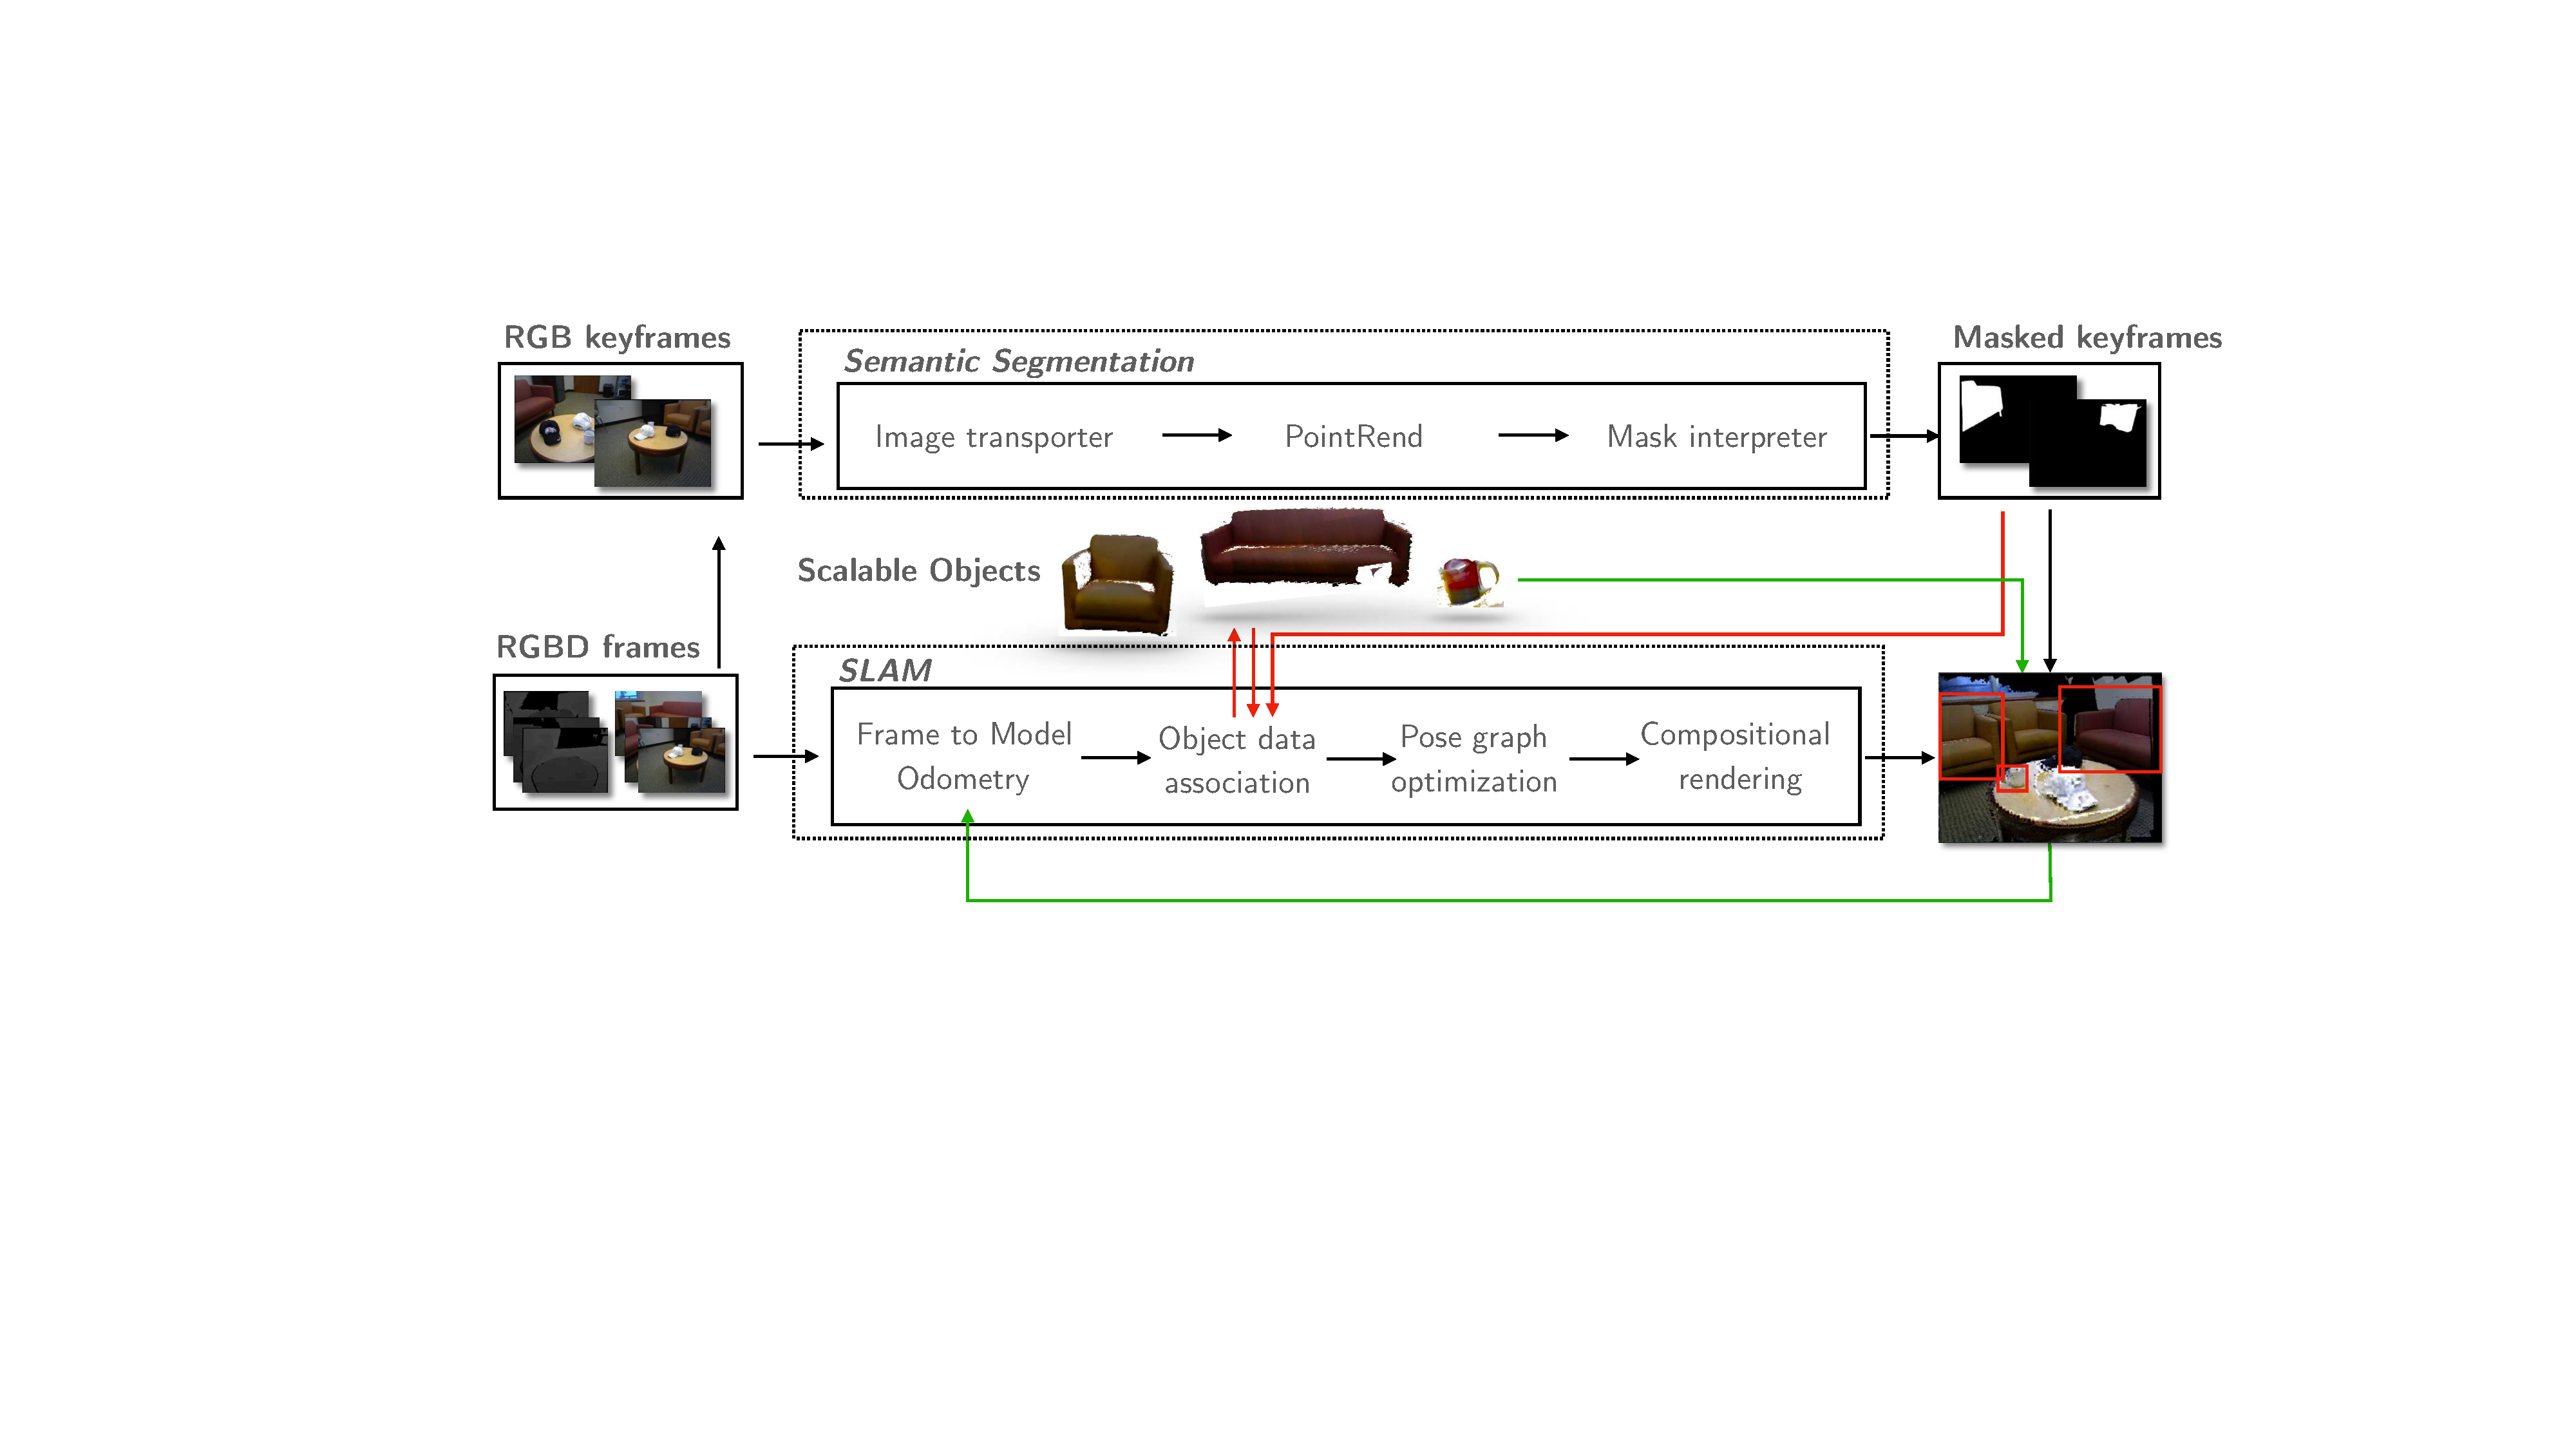
\includegraphics[width=\linewidth]{figs/icra2021-compressed.pdf}
    \caption{\label{fig:overview} System overview: Top shows the deep object segmentation pipeline that runs asynchronously, Masked keyframes from the segmentation pipeline are used in Data association and map update (shown with red lines). Bottom shows the major stages of the reconstruction system, specifically object models are used in tracking via compositional raycasting (shown with green lines).}
 \end{figure*}

\subsection{Core concepts and notations} \label{subsec: notation}
A background volume $V_B$ is a spatially-hashed voxel grid on GPU, where small $16^3$ subvolumes are allocated around observed 3D points. It is created and updated as a \textit{temporary} instance for stable tracking. An object volume $V_{O_i}$ is akin to the background volume, but persistently maintains the object label, ID, and corresponding object descriptors.

A 3D volume $V$'s properties, including surface vertex positions, normals, and colors, can be mapped to 2D images given a camera pose $\mathbf{T} \in SE(3)$ and camera intrinsics defined as $K$ with ray-casting. We denote such \textit{rendered images} by \( \langle \mathcal{N}, \mathcal{V}, \mathcal{C} \rangle \)  for normal, vertex, and color maps respectively. They can be associated with \textit{input RGB-D images} $\langle \mathcal{I}, \mathcal{D}\rangle $ that consist of color ($\mathcal{I}$) and depth ($\mathcal{D}$) images via projective closest points.

We use subscripts and superscripts to indicate multiple coordinate frames used in our pipeline, including $C_i$ for $i$th camera, $O_j$ for $j$th object, and $W$ for background or world coordinate frame. For instance,
\(\langle \mathcal{N}_{C_s}, \mathcal{V}_{C_s}, \mathcal{C}_{C_s} \rangle \) represents 2D maps rendered from the volumes in the $C_s$ camera coordinate frame.
$\mathbf{T}_{O_j}^W \in SE(3)$ encodes a rigid transformation from object $j$ to world. Finally, we denote the respective measurements between nodes with variable $\mathbf{Z}$.

\subsection{Hybrid frame-to-model odometry} \label{subsec: tracking}

In \textit{RGB-D} camera tracking, we seek to estimate the relative camera pose \(\mathbf{T}^{C_t}_{C_s}\) given an incoming \textit{RGB-D} target frame \( \langle \mathcal{I}_{C_t}, \mathcal{D}_{C_t}\rangle \) and a source model \( \langle \mathcal{N}_{C_{s}}, \mathcal{V}_{C_{s}}, \mathcal{C}_{C_{s}}\rangle \) of the scene rendered by placing a virtual camera at the previous camera frame ${C_s}$.

We accomplish this by minimizing the joint weighted dense geometric error residual $r_D$ and the photometric error residual $r_I$. The general energy function is formulated as in \cite{park_colored_2017} by accumulating residual at every point $p \in \mathbb{R}^2$ with a valid data association:
\begin{align}
    E(\mathbf{T}^{C_t}_{C_{s}}) = \sum_{p} (1 - \sigma) r_I^2(\mathbf{T}^{C_t}_{C_s}, p) + \sigma r_D^2(\mathbf{T}^{C_t}_{C_s}, p), \label{eq:1}
\end{align}
Here, we adapt the geometric ICP residual as the point-to-plane distance between the incoming depth map $\mathcal{D}$ and the rendered vertex and normal map $(\mathcal{V}_{C_s}, \mathcal{N}_{C_s})$ as follows, using the formulation in \cite{newcombeKinectFusionRealtimeDense2011}:
\begin{align}
    r_D(T^{C_t}_{C_s}, p) = \bigg((T^{C_t}_{C_{s}} \mathcal{V}_{C_s}( \hat{p} ) - \mathcal{V}_{C_{t}}(p )\bigg) \cdot \mathcal{N}_{C_{t}}( p ), \label{eq:2}
\end{align}
where $\mathcal{V}_{C_t}$ is the vertex map from unprojecting the input depth image $\mathcal{D}_{C_t}$.
Additionally, we use a photometric error residual to improve tracking robustness, which is defined as:
\begin{align}
    r_I(T^{C_t}_{C_s}, p) = \mathcal{C}_{C_s}(\hat{p}) - \mathcal{I}_{C_t}(p). \label{eq:3}
\end{align}
In equations (\ref{eq:2}) and (\ref{eq:3}), $\hat{p}$ is the correspondence of $p$ in the source frame, and is computed via \textit{warping}:
\begin{align}
    \hat{p} = K {\mathbf{T}^{C_t}_{C_s}}^{-1}\mathcal{D}_{C_t}(p)K^{-1}[p^\top, 1]^\top. \label{eq:4}
\end{align}
It must be noted that the $p$s are a subset of pixels with valid object-level data associations detailed in \S\ref{subsec: rendering}.

The energy function in equation \ref{eq:1} is minimized using the Gauss-Newton algorithm. We implement the minimization in a coarse to fine scheme using an image pyramid, on the GPU in parallel since each pixel acts independently in the energy function using \textit{reduction} with appropriate thread conflict handling as described in \cite{dongGPUAcceleratedRobust2019}.



\subsection{Object instance segmentation and association} \label{subsec: segmentation}

\textbf{2D instance segmentation:} Object detection and instance masks are generated every $n^{th}$ frame (we choose $n=10$) in a separate thread from the \textit{PointRend} backend. \textit{PointRend} uses a Resnet-50-FPN backbone network to generate a convolutional feature map. In particular, after an empirical evaluation, we found that \textit{PointRend} provided better masks over \textit{Mask-RCNN}.

The semantic segmentation module maps incoming \textit{RGB} frame \(\mathcal{I}\) into a set of object labels $[l_1, \dots l_k]$, a set of binary object masks $M_n^i$ defined over $l \in \mathcal{L} \triangleq \{0, \dots, L_{max}-1\}$ object classes ($L_{max}=80$ in the MS-COCO dataset), bounding boxes $b \in \mathbb{N}^4$, and a probability distribution $p(l_i \mid \mathcal{I})$. We also extract the object feature map for the accepted object proposals, from the penultimate fully connected layer of the R-CNN from the object classifier head. We observe that these feature maps provide us with robust data association in ambiguous situations.
%
To obtain instance segmentation for frames not sent to the DNN, we warp the binary mask images from the most recent frame with a segmentation and fill the holes in the warped masks using the \textit{flood fill} algorithm.

Once the current camera pose and the semantic segmentation information are available, instance detections are associated with existing objects. Unmatched instance detections are used to initialize new object volumes.

\textbf{3D instance generation:} When an unmatched object is to be instantiated, the masked depth frame at $C_i$ is unprojected and transformed into the world frame to obtain the object point cloud:
\begin{align}
X_{W} = \mathbf{T}^W_{C_i} K^{-1} D_{C_i}(p) [p^\top, 1]^\top.
\end{align}
To obtain relatively high fidelity reconstruction, we adaptively calculate a conservative voxel length of
\begin{align}
    l = \gamma \| \max(X_W) - \min(X_W) \|_{\infty},
\end{align}
where $\min, \max$ operators are applied to all dimensions of $X \in \mathbb{R}^3$ simultaneously. We empirically use $\gamma = 1 / 64\sqrt{2}$, but due to the scalability of the volume our model is less sensitive to $\gamma$.
Finally, the object pose is simply chained by
\begin{align}
    \mathbf{T}_{O}^W = \mathbf{T}_{C_i}^{W} \bigg({\mathbf{T}_{C_i}^O}\bigg)^{-1},
\end{align}
where $\mathbf{T}_{C_i}^O = [I \mid t_{C_i}^O]$ with $t_{C_i}^O = \min(X_W) - t_{C_i}^W $. Each new object is also initialized with the object feature map from its corresponding instance mask.

\textbf{2D--3D semantic data association:}
To associate existing object volumes to 2D instances, visible objects are rendered (in \S\ref{subsec: rendering}) in the current frame. The rendered color map $\mathcal{C}$ is thresholded to obtain a virtual binary mask. An intersection over union (IoU) between the virtual binary mask $\hat{\mathcal{M}}$ and the instance masks $\mathcal{M}_i$ in the current frame is used as a scoring metric as defined in \cite{mccormacFusionVolumetricObjectLevel2018}.

As opposed to computing the $\argmax_{i}{\text{IoU}(\mathcal{M}_i, \hat{\mathcal{M})}}$, we associate objects as given below:
\begin{align}
    i = \argmin_{i \in \mathcal{S}} (\| f_i - \hat{f} \|_1),
\end{align}
where $\hat{f}$ and $f_i$ denote feature map of the object render (identical to the object in question), and the instance masks respectively and $\mathcal{S} \triangleq \{i : \text{IoU}(\mathcal{M}_i, \hat{M}) > 0.2\}$.
Associating object renders to instance masks in this manner prevents incorrectly fusing object instances between nearby similar objects, in cases where there is large accumulated drift.

% In practice, we reuse the object render generated after pose-graph optimization from the previous frame, for improved performance, as \textit{ray-casting} is the largest bottleneck on the system.

For subsequent fusion of a 2D instance detection to its associated 3D object, the instance mask---containing the object foreground---and the bounding box mask---containing both the foreground and background are used. Similar to \cite{mccormacFusionVolumetricObjectLevel2018} we integrate the object in both the foreground and background through a weighted average of TSDF, color, and additionally maintain binomial foreground-background count variables for each voxel. This smoothes out artifacts from integration of 2D instances with spurious masks.

Finally, we update the object feature map by a gated weight average:
\begin{align}
    f_t = \frac{w_{t-1} \cdot f_{t-1} + \mathcal{H}(f_{t-1}, f_{in}) \cdot f_{in}}{w_{t-1} + \mathcal{H}(f_{t-1}, f_{in})},\\
    \mathcal{H}(f_{t-1}, f_{in}) = \frac{\textrm{sgn}(\lambda - ||f_{t-1} - f_{in}||_1) + 1}{2},
\end{align}
where $\mathcal{H}$ is the Heaviside step function that hard-filters outlier input feature map $f_{in}$ compared to the maintained object feature map $f_{t-1}$ with weight $w_{t-1}$ controlled by the threshold $\lambda$.

\subsection{Factor graph optimization} \label{subsec: optimization}
As we have mentioned before, a background volume is maintained for stable tracking, and to handle \textit{objectless} frames. The background volume, additionally maintains the ratio ($r$) of visible volume units in the current camera frustum to the total number allocated volume units in the volume. A low ratio implies that the camera may have moved away from a particular part of the scene. Pose graph optimization is conditionally triggered when the background volume is reset owing to low ratio of visible units ($r < 0.2$) and when there are new objects added into the graph.

Our object factor graph formulation is similar to \cite{salas-morenoSLAMSimultaneousLocalisation2013, mccormacFusionVolumetricObjectLevel2018}. The variable nodes $\mathcal{X} = \{\mathbf{x}_1, \dots \mathbf{x}_N\}$ are partitioned into camera pose variables $\mathbf{T}^{W}_{C_i} \in SE(3)$ and object pose variables $\mathbf{T}^W_{O_j} \in SE(3)$. The first camera pose is initialized as the world frame $W$.

Assuming a Gaussian noise model, the \textit{MAP} inference problem with the above variable nodes reduces to solving the following non-linear least squares optimization:
\begin{multline}
    \mathcal{X}^* = \argmin_{\mathcal{X}} \Big( \sum_{k \in |C|} \|  \mathbf{Z}^{C_k}_{C_{k-1}} \ominus \mathbf{T}^{C_k}_{C_{k-1}} \|_{\Sigma_{k,k-1}}^2 \\
    + \sum_{j \in |\mathcal{O}|, k \in |\mathcal{C}|} \| \mathbf{Z}^{O_j}_{C_k} \ominus \mathbf{T}^{O_j}_{C_k} \|_{\Sigma_{o_j, k}}^2 \Big),
\end{multline}
where the operator $ \mathcal{Y} \ominus \mathcal{X} = \text{Log}(\mathcal{X}^{-1} \mathcal{Y})$ expresses the relative error in the local tangent vector space \cite{solaMicroLieTheory2020}. $\Sigma_{k, k-1}$ denotes the covariance between relative camera pose measurements,  $\Sigma_{o_j, k}$ is the covariance in the camera to object measurement. They can be approximated by information matrices computed from \textit{odometry}, however, empirically we found that a constant information matrix can achieve reasonable results. We obtain the relative camera measurements $\mathbf{Z}^{C_k}_{C_{k-1}}$ from \textit{frame to model odometry} (\S\ref{subsec: tracking}), and obtain frame to object measurements $\mathbf{Z}^{O_j}_{C_k}$ by performing an additional Gauss Newton iteration with only the object pixels. Finally, the expected relative camera pose $\mathbf{T}^{C_k}_{C_{k-1}}$ and expected camera object pose $\mathbf{T}^{O_j}_{C_k}$ used in the factors are calculated as:
\begin{align}
    \mathbf{T}^{C_k}_{C_{k-1}} &= \bigg({\mathbf{T}^{W}_{C_k}}\bigg)^{-1} \mathbf{T}^{W}_{C_{k-1}}, \\
    \mathbf{T}^{O_j}_{C_k} &= \bigg({\mathbf{T}^{W}_{O_j}}\bigg)^{-1} \mathbf{T}^{W}_{C_k}.
\end{align}

We solve the optimization in GTSAM \cite{dellaert2012factor}, using Levenberg Marquardt. Since the entire object volume is transformed as a rigid body, the object volumes remain unchanged in memory after optimization. We note that this circumvents the time-consuming re-integration that usually takes place in volumetric methods after PGO \cite{whelanElasticFusionDenseSLAM2015}.

\subsection{Compositional rendering} \label{subsec: rendering}
Compositional rendering is a serialized operation that generates normal, vertex, and color maps by ray-casting 3D objects in the viewing frustum into 2D object instances, and is illustrated in Figure~\ref{fig:compositional_render}.

\begin{figure}[t!]
    \centering
    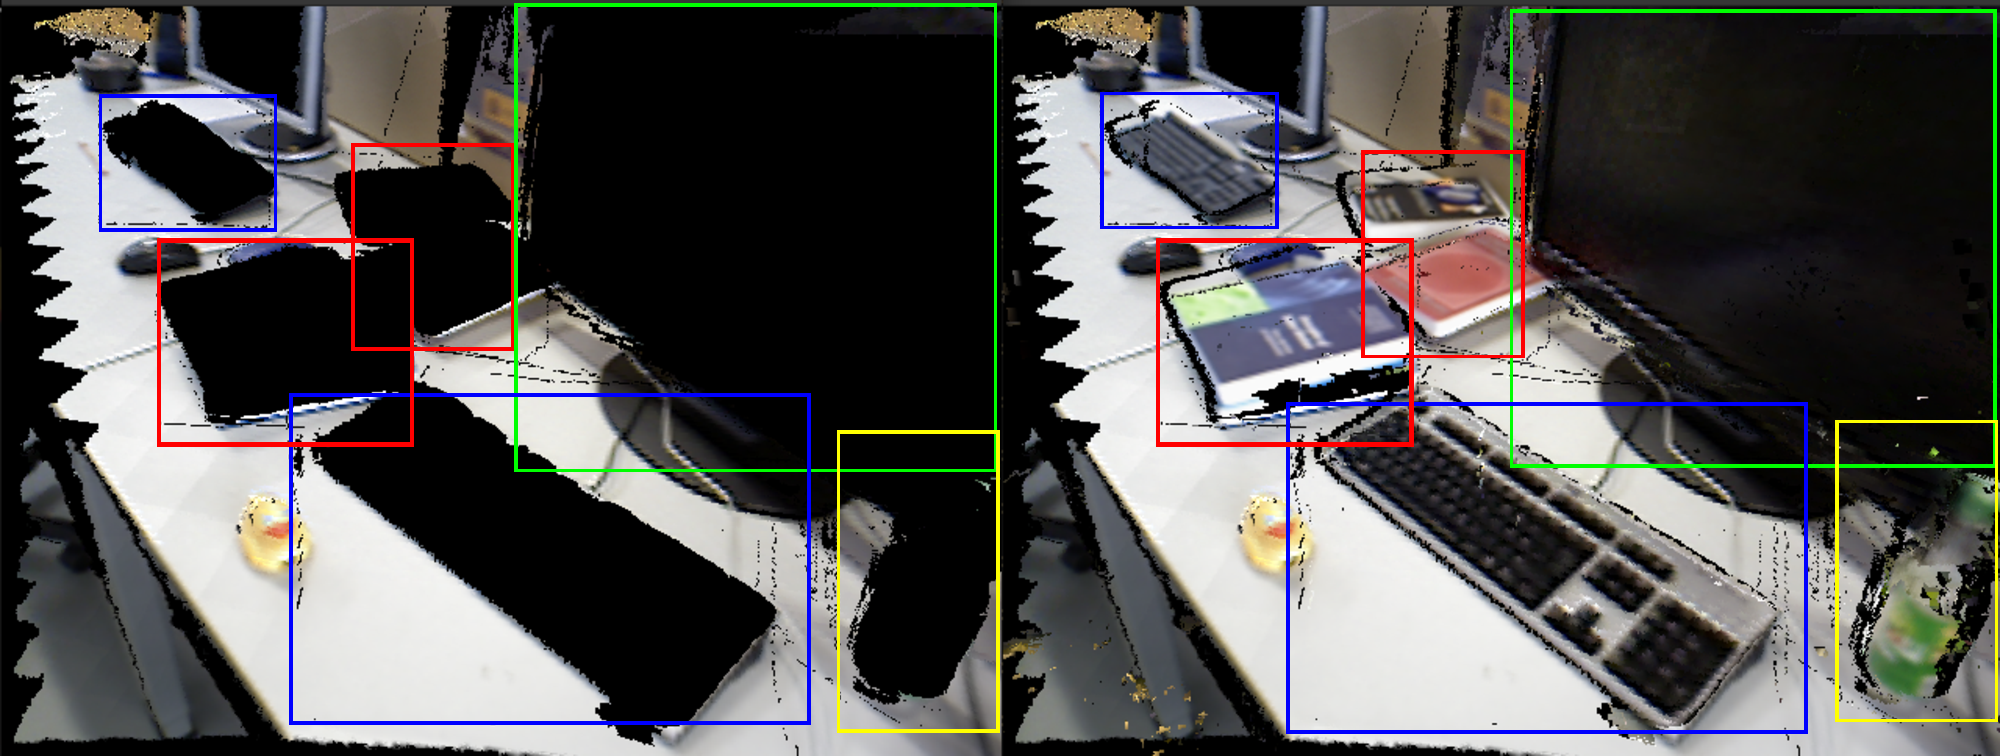
\includegraphics[width=\linewidth]{figs/compositional-render.pdf}\vspace{-5mm}
    \caption{Compositional rendering during reconstruction on TUM \textit{fr3\_long\_office\_household} dataset. Left shows the background render, and right shows the composed render. Compositionally rendered objects are shown in bounding boxes.}
    \vspace*{-1em}
    \label{fig:compositional_render}
\end{figure}

\(\langle \mathcal{N}_{C_i}, \mathcal{V}_{C_i}, \mathcal{C}_{C_i} \rangle \) is in fact an aggregation of separate renderings from object volumes \(\langle \mathcal{N}_{C_i}^{V_{{O}_j}}, \mathcal{V}_{C_i}^{V_{{O}_j}}, \mathcal{C}_{C_i}^{V_{\mathcal{O}_j}} \rangle \) and the background volume \(\langle \mathcal{N}_{C_i}^{V_{B}}, \mathcal{V}_{C_i}^{V_{B}}, \mathcal{C}_{C_i}^{V_{{B}}}  \rangle \), depending on the masks. In particular, we render the background volume, based on a background mask that is constructed from the union of existing virtual object masks in the current frame, and associated instance masks.

Then, the composed per-pixel map model render can be obtained as follows:
\begin{align}
    &\hat{k} = \argmin_k \mathcal{V}_k(p)[z], ~k \in \{O_1, \cdots, O_n, B\} \\
    &\langle \mathcal{N}^*(p), \mathcal{V}^*(p), \mathcal{C}^*(p) \rangle = \langle  \mathcal{N}_{\hat{k}}(p), \mathcal{V}_{\hat{k}}(p), \mathcal{C}_{\hat{k}}(p) \rangle,
\end{align}
where $\hat{k}$ is the volume index corresponding to the minimum distance to camera center for pixel $p$.

Object volumes not currently visible are downloaded from GPU into CPU memory. Note that downloading the object volume does not affect the optimization problem, since the object volumes are required only for integration and raycasting.


% -*- mode:LaTex; mode:visual-line; mode:flyspell; fill-column:75-*-

\chapter{Conclusions} \label{chapConclusions}

In conclusions, robots are the best.



% \appendix
% % -*- mode:LaTex; mode:visual-line; mode:flyspell; fill-column:75-*-

\chapter{Stuff I forgot} \label{chapAppendix}

Robots are really, really great.

\todo{Add frame to model ICP background??}


% ********************************************************************************
%                                 Back Matter
% ********************************************************************************

\backmatter

% Normal line spacing
\singlespace

% By default \bibsection is \chapter*, but we really want this to show
% up in the table of contents and pdf bookmarks.
\renewcommand{\bibsection}{\chapter{\bibname}}
% Additionally, redefine the chapter header to remove the chapter number.
\renewcommand{\chaptermark}[1]{%
  \markboth{\color{headergray}{#1}}{}
}


%\newcommand{\bibpreamble}{This text goes between the ``Bibliography''
%  header and the actual list of references}
\bibliographystyle{plainnat}

% No whitespace allowed in the reference files list, ever.
% \bibliography{bibliography/references}
\bibliography{bibliography/references_zotero}
\end{document}
